\documentclass[14pt,a4paper]{extarticle}

\usepackage{cmap}
\usepackage[T2A]{fontenc}
\usepackage[utf8]{inputenc}
\usepackage[english,russian,ukrainian]{babel}
\usepackage[metapost,truebbox,mplabels]{mfpic}
\usepackage{listcorr}
\usepackage{epigraph}
\usepackage{floatflt}
\usepackage{multicol}
\usepackage{longtable}
\usepackage{graphicx}
\usepackage{color}
\usepackage{textcomp}
\usepackage{amstext}
\usepackage{amsmath}
\usepackage{amssymb}
\usepackage{amsfonts}
\usepackage{verbatim}
\usepackage{alltt}

% \twocolumn

% \usepackage[landscape,russian]{olymppp}

\usepackage[ukrainian]{olymppp}

\usepackage{anysize}

\def\dib#1{\,#1\discretionary{}{\mbox{$#1$}}{}\,}

\marginsize{20mm}{20mm}{7mm}{20mm}


\renewcommand{\baselinestretch}{1.3125}

\opengraphsfile{pics}

\begin{document}

\def\<{\leqslant}
\def\>{\geqslant}
\def\*{\times}
\def\dib#1{\,#1\discretionary{}{\mbox{$#1$}}{}\,}
\def\op{\mathop{\rm op}\nolimits}
\def\bdiv{\mathop{\rm div}\nolimits}
\def\opt{\mathop{\rm opt}}
\def\isdiv{\mathbin{\hbox to 0.25em{\hfill\hbox to 0 pt{\raisebox{0pt}{\hss$\cdot$\hss}}\hbox to 0 pt{\raisebox{-.6ex}{\hss$\cdot$\hss}}\hbox to 0 pt{\raisebox{.6ex}{\hss$\cdot$\hss}}\hspace{0.15em}\hfill}\,}}

\newlength{\myparindent}


\newlength{\mytemplen}
\newlength{\mytemplensecond}
\newlength{\mytemplenthird}
\newsavebox{\mypictbox}
\def\myrightfigure#1#2{%
\savebox{\mypictbox}{\noindent{}#2}%
\settowidth{\mytemplen}{\usebox{\mypictbox}}%
\settoheight{\mytemplenthird}{\usebox{\mypictbox}}%
\ifdim\mytemplen<0.8\textwidth%
\noindent%
\setlength{\mytemplensecond}{\textwidth}%
\addtolength{\mytemplensecond}{-\mytemplen}%
\addtolength{\mytemplen}{3pt}% ??? better to find alike standard len
\hspace*{\mytemplensecond}\usebox{\mypictbox}%
\par\vspace*{-0.5\baselineskip}\par%
\vspace*{-\mytemplenthird}
\vspace{-\parskip}
\hangindent=-\mytemplen
\hangafter=-#1
\else
\begin{center}
\usebox{\mypictbox}%
\par
\end{center}
% \vspace{-\baselineskip}
\fi%
}

\def\mytextandpicture#1#2{%
\setlength{\myparindent}{\parindent}%
\savebox{\mypictbox}{\noindent{}#2}%
\settowidth{\mytemplensecond}{\usebox{\mypictbox}}%
\setlength{\mytemplen}{\textwidth}%
\addtolength{\mytemplen}{-\mytemplensecond}%
\addtolength{\mytemplen}{-3mm}%
\noindent\mbox{}\hfill\parbox{\mytemplen}{\hspace*{\myparindent}#1}\hfill\hspace{2.5mm}\hfill\parbox{\mytemplensecond}{\usebox{\mypictbox}}\hfill\mbox{}\\
}

\def\myflfigaw#1{%
\savebox{\mypictbox}{\noindent{}#1}%
\settowidth{\mytemplen}{\usebox{\mypictbox}}%
% \addtolength{\mytemplen}{1mm}%
\ifdim\mytemplen<0.75\textwidth%
\begin{floatingfigure}[r]{\mytemplen}%
\mbox{\noindent%
\usebox{\mypictbox}%
\vspace{-6pt}}
\end{floatingfigure}%
\else
\begin{figure*}[h]%
\usebox{\mypictbox}%
\end{figure*}%
\fi%
}

\def\myhrulefill{\vspace{12mm}\par\vspace*{-12mm}\par\hrulefill}

\newenvironment{problemAllDefault}[1]{\vspace{10mm}\par\begin{problem}{#1}{Клавіатура (stdin)}{Екран (stdout)}{1 сек}{64 мегабайти}}{\end{problem}}


%%% \in%put pseudo-title

\begin{center}

\begin{huge}

~

\vfill

Цю сторінку замінити на сторінку з титулкою, набраною якимись іншими засобами

\vfill

~

\clearpage

~

\vfill

Цю сторінку замінити на сторінку з <<выходными сведениями>>, набраною якимись іншими засобами

\vfill

~

\end{huge}

\end{center}

\clearpage

\contest{Обласна інтернет-олімпіада 2013/14 навч. року}{Черкаська обл.}{08.10.2013}

\section{Обласна інтернет-олімпіада 2013/14 н.~р.}

Задачі доступні для дорішування (\verb"ejudge.ckipo.edu.ua", змагання $\No$10).

\renewenvironment{problemAllDefault}[1]{\vspace{10mm}\par\begin{problem}{#1}{Клавіатура (stdin)}{Екран (stdout)}{1 сек}{64 мегабайти}}{\end{problem}}

\begin{problemAllDefault}{Тор}

Як відомо, \emph{тор}\nolinebreak[3] --- це поверхня бублика, яку можна отримати таким чином: узяти прямокутник розміром $n$~клітинок по~вертикалі на $m$~клітинок по~горизонталі, склеїти верхню сторону з нижньою (отримається циліндр), потім закрутити циліндр у бублик і склеїти ліву сторону з правою.

\parbox{100pt}{%
\begin{mfpic}[2]{0}{50}{0}{20}
\pen{2pt}
\polygon{(0,0),(10,20),(50,20),(40,0)}
\pen{0.5pt}
\lines{(0.5 , 1),(40.5, 1)}
\lines{(1   , 2),(41  , 2)}
\lines{(1.5 , 3),(41.5, 3)}
\lines{(2   , 4),(42  , 4)}
\lines{(2.5 , 5),(42.5, 5)}
\lines{(3   , 6),(43  , 6)}
\lines{(3.5 , 7),(43.5, 7)}
\lines{(4   , 8),(44  , 8)}
\lines{(4.5 , 9),(44.5, 9)}
\lines{(5   ,10),(45  ,10)}
\lines{(5.5 ,11),(45.5,11)}
\lines{(6   ,12),(46  ,12)}
\lines{(6.5 ,13),(46.5,13)}
\lines{(7   ,14),(47  ,14)}
\lines{(7.5 ,15),(47.5,15)}
\lines{(8   ,16),(48  ,16)}
\lines{(8.5 ,17),(48.5,17)}
\lines{(9   ,18),(49  ,18)}
\lines{(9.5 ,19),(49.5,19)}
\arrow[l5]\reverse\arrow[l5]\ellipse[-30]{(0,10),2,5}
\end{mfpic}}%
\hfill\hfill\hfill%
\begin{Huge}$\Rightarrow$\end{Huge}
\hfill\hfill\hfill%
\parbox{120pt}{%
\begin{mfpic}[1.6]{0}{70}{0}{10}
\pen{1pt}
\ellipse{(5,5),2,5}
\fillcolor{gray(0.75)}
\gfill\ellipse{(5,5),2,5}
\curve{
(65+2*cosd(-90), 5+5*sind(-90)),
(65+2*cosd(-60), 5+5*sind(-60)),
(65+2*cosd(-30), 5+5*sind(-30)),
(65+2*cosd(  0), 5+5*sind(  0)),
(65+2*cosd( 30), 5+5*sind( 30)),
(65+2*cosd( 60), 5+5*sind( 60)),
(65+2*cosd( 90), 5+5*sind( 90))}
\pen{0.5pt}
\lines{(5+2*cosd(-90), 5+5*sind(-90)),  (65+2*cosd(-90), 5+5*sind(-90))}
\lines{(5+2*cosd(-72), 5+5*sind(-72)),  (65+2*cosd(-72), 5+5*sind(-72))}
\lines{(5+2*cosd(-54), 5+5*sind(-54)),  (65+2*cosd(-54), 5+5*sind(-54))}
\lines{(5+2*cosd(-36), 5+5*sind(-36)),  (65+2*cosd(-36), 5+5*sind(-36))}
\lines{(5+2*cosd(-18), 5+5*sind(-18)),  (65+2*cosd(-18), 5+5*sind(-18))}
\lines{(5+2*cosd(  0), 5+5*sind(  0)),  (65+2*cosd(  0), 5+5*sind(  0))}
\lines{(5+2*cosd( 18), 5+5*sind( 18)),  (65+2*cosd( 18), 5+5*sind( 18))}
\lines{(5+2*cosd( 36), 5+5*sind( 36)),  (65+2*cosd( 36), 5+5*sind( 36))}
\lines{(5+2*cosd( 54), 5+5*sind( 54)),  (65+2*cosd( 54), 5+5*sind( 54))}
\lines{(5+2*cosd( 72), 5+5*sind( 72)),  (65+2*cosd( 72), 5+5*sind( 72))}
\lines{(5+2*cosd( 90), 5+5*sind( 90)),  (65+2*cosd( 90), 5+5*sind( 90))}
\begin{coords}
\reflectabout{(30,10)}{(40,20)}
\arrow[l5]\reverse\arrow[l5]\ellipse{(35,15),2,5}
\end{coords}
\end{mfpic}}%
\hfill\hfill\hfill%
\begin{Huge}$\Rightarrow$\end{Huge}
\hfill\hfill\hfill% 
\parbox{120pt}{%
\begin{mfpic}[1]{-50}{50}{-30}{30}
\yscale{0.4}
\arc[p]{(0,25*sind(288)), 60,120,(50-10*cosd(288))}
\arc[p]{(0,25*sind(306)), 28,152,(50-10*cosd(306))}
\arc[p]{(0,25*sind(324)), 20,160,(50-10*cosd(324))}
\arc[p]{(0,25*sind(342)), 12,168,(50-10*cosd(342))}
\arc[p]{(0,25*sind(  0)),  3,177,(50-10*cosd(  0))}
\arc[p]{(0,25*sind( 18)),-10,190,(50-10*cosd( 18))}
\arc[p]{(0,25*sind( 36)),-20,200,(50-10*cosd( 36))}
\arc[p]{(0,25*sind( 54)),-50,230,(50-10*cosd( 54))}
\circle{(0,25*sind( 72)),(50-10*cosd( 72))}
\circle{(0,25*sind( 90)),(50-10*cosd( 90))}
\circle{(0,25*sind(108)),(50-10*cosd(108))}
\arc[p]{(0,25*sind(126)),135,405,(50-10*cosd(126))}
\arc[p]{(0,25*sind(144)),155,385,(50-10*cosd(144))}
\arc[p]{(0,25*sind(162)),165,375,(50-10*cosd(162))}
\arc[p]{(0,25*sind(180)),172,368,(50-10*cosd(180))}
\arc[p]{(0,25*sind(198)),180,360,(50-10*cosd(198))}
\arc[p]{(0,25*sind(216)),190,350,(50-10*cosd(216))}
\arc[p]{(0,25*sind(234)),200,340,(50-10*cosd(234))}
\arc[p]{(0,25*sind(252)),225,315,(50-10*cosd(252))}
\end{mfpic}}%
\hfill~\\                                 

Назвемо дві клітинки \emph{сусідніми}, якщо вони мають спільну сторону. Нехай за\nolinebreak[2] одну секунду можна перейти з\nolinebreak[2] клітинки до\nolinebreak[2] будь-якої сусідньої з~нею. За~який мінімальний час можна потрапити з\nolinebreak[2] клітинки\nolinebreak[2] $(r_1; c_1)$ у\nolinebreak[2] клітинку\nolinebreak[2] $(r_2; c_2)$? Перше число у\nolinebreak[2] позначенні клітинки\nolinebreak[3] --- номер рядка початкового прямокутника, друге\nolinebreak[3] --- номер стовпчика.

\InputFile  Програма повинна прочитати зі\nolinebreak[3] стандартного входу (клавіатури) шість натуральних чисел, у~порядку $n$,~$m$, $r_1$,~$c_1$,\nolinebreak[2] $r_2$,~$c_2$. 
Виконуються обмеження: $2\dib{{\<}}{n, m}\dib{{\<}}{1\,000\,000\,000}$,\hspace{1em plus 2em}\linebreak[1]$1\dib{{\<}}{r_1, r_2}\dib{{\<}}n$,\hspace{1em plus 2em}\linebreak[1]$1\dib{{\<}}{c_1,c_2}\dib{{\<}}m$.

\OutputFile Програма має вивести на стандартний вихід (екран) єдине ціле число\nolinebreak[3] --- мінімальний час.

\Examples
\begin{exampleSimple}{7em}{3em}%
\exmp{10 10 5 5 1 1}{8}%
\exmp{10 10 9 9 1 1}{4}%
\end{exampleSimple}


\end{problemAllDefault}
	

{\hyphenpenalty=400

\Tutorial	Необхідно дістатися з точки $(r_1, c_1)$ у~точку $(r_2, c_2)$ по <<зацикленому>> простору. 
Скориставшися відомим принципом незалежності переміщень, можна побачити, що переміщення в горизонтальному і вертикальному напрямках не~залежать одне від одного. Зрозуміти це можна, розглядаючи переміщення як перетин вертикальних і горизонтальних сторін клітинки. Не~залежно від траєкторії необхідно перетнути лише певну конкретну кількість вертикальних ліній (позначимо цю кількість~$\Delta{}r$) і горизонтальних ліній (відповідно~$\Delta{}c$). (Звісно, маючи на\nolinebreak[3] увазі, що ми не\nolinebreak[3] розглядаємо відверто не\nolinebreak[3] мінімальні шляхи, де одна й та ж горизонтальна чи вертикальна лінія перетинається багатократно.) Тоді відповідь на задачу є ${\Delta{}r+\Delta{}c}$, оскільки для зміни будь якої з координат на~1 необхідно затратити 1~секунду.

Є 2 способи переміститися з рядка $r_1$ у~$r_2$\nolinebreak[3] --- перетинаючи край початкового (до згинів і склеювань) прямокутника і не~перетинаючи. Вважаємо спочатку, що ${r_1{<}r_2}$. Тоді не~перетинаючи край витратимо ${(r_2{-}r_1)}$\nolinebreak[2] сек, а~перетинаючи спочатку доберемося до рядка~1 (${(r_1{-}1)}$\nolinebreak[2] сек),  потім до\nolinebreak[1] рядка~$n$ (1~сек), і\nolinebreak[2] з\nolinebreak[2] нього у\nolinebreak[3] $r_2$\nolinebreak[3] --- (${(n{-}r2)}$\nolinebreak[2] сек). Сумарно ${(r_1{-}r_2{+}n)}$\nolinebreak[2] сек. 
Тобто, треба вибрати мінімум зі значень ${(r_2{-}r_1)}$ (не~перетинаючи край) і\nolinebreak[3] ${(r_1{-}r_2{+}n)}$ (через\nolinebreak[3] край). Але це лише для випадку ${r_1{<}r_2}$, а\nolinebreak[3] при ${r_1{>}r_2}$ аналогічними міркуваннями отримуються схожі, але інші формули ${(r_1{-}r_2)}$ і\nolinebreak[3] ${(r_2{-}r_1{+}n)}$. Щоб\nolinebreak[2] не\nolinebreak[2] задумуватися, яка з\nolinebreak[3] координат більша, можна використати формулу
$$
\Delta{}r \, = \, \min\bigl((r1-r2+n) \bmod n, (r2-r1+n) \bmod n\bigr)
$$
З~$\Delta{}c$ слід вчинити аналогічно, потім додати ${\Delta{}r+\Delta{}c}$.

}


\begin{problemAllDefault}{Паркет--1}

{\tolerance=9999

Щоб зобразити за допомогою паркету Супер-Креативний Візерунок, треба\linebreak[1]
$N_1$\nolinebreak[3] дощечок розмірами\nolinebreak[2] $1{\*}1$,\linebreak[1]
$N_2$\nolinebreak[3] дощечок розмірами\nolinebreak[2] $2{\*}1$,\linebreak[1]
$N_3$\nolinebreak[3] розмірами\nolinebreak[1] $3{\*}1$,\linebreak[1]
$N_4$\nolinebreak[4] розмірами\nolinebreak[1] $4{\*}1$ та 
$N_5$\nolinebreak[3] дощечок розмірами\nolinebreak[3] $5{\*}1$. 
Купити можна лише дощечки розмірами\nolinebreak[2] $5{\*}1$. Дощечки можна різати, але не~можна склеювати. Наприклад, коли потрібні п’ять дощечок $2{\*}1$, їх не~можна зробити з двох дощечок $5{\*}1$, але можна з трьох. Для цього дві з них розріжемо на три частини $2{\*}1$, $2{\*}1$ та $1{\*}1$ кожну, а третю\nolinebreak[3] --- на дві частини $2{\*}1$ та $3{\*}1$. Отримаємо потрібні п’ять дощечок $2{\*}1$, а дві дощечки $1{\*}1$ та одна $3{\*}1$ підуть у відходи.

}

Напишіть програму, яка, прочитавши кількості дощечок $N_1$, $N_2$, $N_3$, $N_4$ та\nolinebreak[3] $N_5$, знайде, яку мінімальну кількість дощечок $5{\*}1$ необхідно купити.

\InputFile	слід прочитати зі стандартного входу (клавіатури). Це будуть п’ять чисел $N_1$, $N_2$, $N_3$, $N_4$ та $N_5$ (саме в такому порядку), розділені пропусками (пробілами).

\OutputFile	Єдине число (скільки дощечок треба купити) виведіть на стандартний вихід (екран).


\Examples
\begin{exampleSimple}{5em}{3em}%
\exmp{0 5 0 0 0}{3}%
\exmp{1 1 1 1 1}{3}%
\end{exampleSimple}

\Scoring	Усі кількості невід’ємні; 90~балів (з~250) припадатиме на\nolinebreak[3] тести, в~яких сумарна кількість $N_1\dib{{+}}N_2\dib{{+}}N_3\dib{{+}}N_4\dib{{+}}N_5$ перебуває в межах від 0 до 20, ще~80~балів\nolinebreak[3] --- від 100 до 10 000, решта 80~балів\nolinebreak[3] --- від 500 000 000 до 2 000 000 000. 

Здати потрібно одну програму, а не для кожного випадку окремо; різні обмеження вводяться виключно для того, щоб дати приблизне уявлення, скільки балів можна отримати, розв’язавши задачу не повністю.



\end{problemAllDefault}
	

\Tutorial	Задача досить складна тим, що треба дуже акуратно розглянути всі випадки, і разом з тим дуже проста тим, що для остаточної реалізації програми не\nolinebreak[3] потрібні ніякі засоби, крім розгалужень та присвоєнь. 

Нехай змінні \texttt{n1}, \texttt{n2}, \texttt{n3}, \texttt{n4} та \texttt{n5} містять потрібні кількості дощечок розмірами $1{\*}1$, $2{\*}1$, $3{\*}1$, $4{\*}1$ та $5{\*}1$ відповідно, у змінній \texttt{res} будемо будувати відповідь задачі. Протягом роботи алгоритму значення деяких зі змінних \texttt{n1}, \texttt{n2}, \texttt{n3}, \texttt{n4} або \texttt{n5} можуть зменшуватися — по мірі того, як враховуємо відповідні кількості у змінній \texttt{res}, яка наприкінці міститиме остаточну відповідь. 






{

\def\leftColumnWidth{0.35\textwidth}
\def\rightColumnWidth{0.6\textwidth}
\def\leftCell#1{\ttfamily\obeylines\obeyspaces\frenchspacing
\begin{minipage}[t]{\leftColumnWidth}
{\ttfamily\obeylines\obeyspaces\frenchspacing #1}
\end{minipage}}
\def\rightCell#1{
\begin{minipage}[t]{\rightColumnWidth}
{#1}
\end{minipage}\medskip}

\def\tabbb{\hspace*{2em}}

\begin{longtable}{|p{\leftColumnWidth}|p{\rightColumnWidth}|}
\hline
\multicolumn{1}{|c|}{Фрагмент коду} 
&
\multicolumn{1}{|c|}{Коментар}
\\\hline\endhead

\leftCell{res = n5}
&
\rightCell{На кожну дощечку розмірами $5{\*}1$ неминуче потрібна окрема ціла дощечка.}
\\\hline

\leftCell{res += n4}
&
\rightCell{На кожну дощечку розмірами $4{\*}1$ теж неминуче потрібна окрема дощечка\dots}
\\\hline

\leftCell{n1 -= min(n1,n4)}
&
\rightCell{\dots{}але обрізки після відрізань дощечок розмірами $4{\*}1$ можна використати як дощечки розмірами $1{\*}1$. Тому надалі можна вважати, що потреба в дощечках $1{\*}1$ складає вже не \texttt{n1}, а або \texttt{n1–n4}, або~\texttt{0}.}
\\\hline

\leftCell{res += n3}
&
\rightCell{На кожну дощечку розмірами $3{\*}1$ теж неминуче потрібна окрема дощечка\dots}
\\\hline

\leftCell{if (n2>n3):\\
\tabbb{}n2 -= n3}
&
\rightCell{\dots{}причому, при $N_2{>}N_3$ просто використовуємо всі обрізки як дощечки розмірами $2{\*}1$\dots}
\\\hline

\leftCell{else:\\
\tabbb{}n3 -= n2\\
\tabbb{}n2 = 0\\
\tabbb{}n1 -= min(n3*2, n1)}
&
\rightCell{\dots{}а при $N_2{\<}N_3$ спочатку формуємо з цих обрізків абсолютно всі дощечки $2{\*}1$, а із решти — ще й min(n3*2, n1) дощечок $1{\*}1$.}
\\\hline

\leftCell{res += n2/2\\
\tabbb{}n1 -= min(n1,n2/2)\\
\tabbb{}n2 \%= 2}
&
\rightCell{Оскільки всі дощечки розміром $3{\*}1$ раніше вже сформовані, то тепер на кожну пару дощечок розміром $2{\*}1$ неминуче потрібна окрема дощечка, причому обрізок можна використати як дощечку $1{\*}1$.\\
\emph{Ділення тут цілочисельне (div).}}
\\\hline

\leftCell{if n2==1:\\
\tabbb{}res += 1\\
\tabbb{}n1 -= min(n1,3)\\
\tabbb{}n2 = 0}
&
\rightCell{Якщо при виконанні попереднього етапу кількість дощечок розміром $2{\*}1$ була непарна, то зараз треба сформувати останню дощечку розміром $2{\*}1$, причому обрізок можна використати для формування від нуля до трьох дощечок розмірами $1{\*}1$.}
\\\hline

\leftCell{res += n1/5\\
\tabbb{}n1 \%= 5}
&
\rightCell{Якщо, незважаючи на усі попередні кроки, досі є потреба в дощечках розміром $1{\*}1$, формуємо їх, розрізаючи кожну дощечку на 5 частин.\\
\emph{Ділення тут цілочисельне (div).}}
\\\hline


\leftCell{if n1 > 0:\\
\tabbb{}res += 1}
&
\rightCell{Якщо після попереднього кроку все ще залишилася потреба у дощечках розміром $1{\*}1$ (від 1 до 4 штук), дя цього достатньо ще\nolinebreak[2] \emph{однієї} дощечки $5{\*}1$.}
\\\hline
\end{longtable}



}

(Мова коду\nolinebreak[3] --- Python;\hspace{0.5em plus 1em}\linebreak[1]
``\verb"="'' (одинарне)\nolinebreak[3] --- присвоєння;\hspace{0.5em plus 1em}\linebreak[1]
``\verb"=="'' (подвійне)\nolinebreak[3] --- перевірити, чи\nolinebreak[3] дорівнює;\hspace{0.5em plus 1em}\linebreak[1]
``\verb"%"''\nolinebreak[3] --- залишок від ділення (\texttt{mod});\hspace{0.5em plus 1em}\linebreak[1]
``\verb"a+=b"''\nolinebreak[3] --- те\nolinebreak[2] само, що \verb"a=a+b", тобто до старого значення~\verb"a" додати~\verb"b" і покласти результат у\nolinebreak[1] ту\nolinebreak[2] саму змінну~\verb"a"; аналогічно ``\verb"a-=b"'', ``\verb"a%=b"''.)


% 

	



% 

	






\contest{ІІ (районний/міський) етап 2013/14 навч. року}{Черкаська обл.}{14.12.2013}

\section{ІІ (районний/міський) етап 2013/14 н.~р.}

Задачі доступні для дорішування (\verb"ejudge.ckipo.edu.ua", змагання $\No$14).

\renewenvironment{problemAllDefault}[1]{\vspace{10mm}\par\begin{problem}{#1}{Клавіатура (stdin)}{Екран (stdout)}{1 сек}{64 мегабайти}}{\end{problem}}

\begin{problemAllDefault}{Електричка}

На кожному вагоні електрички є табличка, на якій фарбою написано його номер. Вагони занумеровані натуральними числами\nolinebreak[1] 1,\nolinebreak[2] 2,~\dots,\nolinebreak[2] $N$ (крайній вагон має номер~1, сусідній з ним\nolinebreak[3] --- номер~2, і~т.~д., до\nolinebreak[3] крайнього з протилежного боку вагону, який має номер~$N$). Електричка має кабіни з обох боків, і\nolinebreak[3] може поїхати хоч\nolinebreak[2] \mbox{1-им} вагоном уперед, хоч\nolinebreak[3] \mbox{$N$-им}.

\ifnum\pdfoutput>0
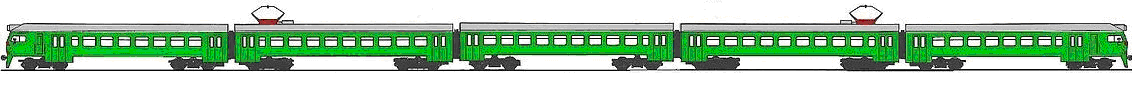
\includegraphics[width=\textwidth,keepaspectratio=true]{elTrain.png}
\else
\fbox{\colorbox{yellow}{Run not latex but pdflatex to insert picture}}
\ifnum\number\month > 6 \ERROR \fbox{Run not latex but pdflatex to insert picture}\fi
\fi

Під час прибуття електрички на платформу, Вітя помітив, що ${(i{-}1)}$ штук вагонів електрички проїхали мимо нього, а\nolinebreak[2] \mbox{$i$-й} по\nolinebreak[2] порядку зупинився якраз навпроти. Ще\nolinebreak[2] він помітив, що\nolinebreak[2] на\nolinebreak[2] табличці цього вагона написаний номер~$j$. Ще\nolinebreak[2] він точно знає (і\nolinebreak[2] ці\nolinebreak[2] знання відповідають дійсності), що\nolinebreak[2] електрички ніколи не\nolinebreak[3] бувають ні\nolinebreak[3] коротшими 4~вагонів, ні\nolinebreak[3] довшими 12~вагонів. Вітя хоче визначити, скільки всього вагонів у\nolinebreak[2] електричці. Напишіть програму, яка або\nolinebreak[2] знаходитиме цю кількість, або\nolinebreak[2] повідомлятиме, що без\nolinebreak[1] додаткової інформації це\nolinebreak[1] зробити неможливо.

\InputFile
Програма має прочитати зі\nolinebreak[3] стандартного входу (клавіатури) два цілі числ\'{а} $i$ та~$j$, розділені пропуском. ${2{\<}i{\<}12}$, ${2{\<}j{\<}12}$, ч\'{и}сла гарантовано задовольняють всі вищезгадані обмеження.

\OutputFile
Виведіть на стандартний вихід (екран) одне число\nolinebreak[3] --- кількість вагонів у\nolinebreak[3] електричці. Якщо однозначно визначити кількість вагонів неможливо, виведіть замість кількості число~\texttt{0}.

\Example
\begin{exampleSimple}{3em}{3em}%
\exmp{4 2}{5}%
\end{exampleSimple}

\end{problemAllDefault}
	

\Tutorial	Розглянемо два випадки: 

\begin{itemize}
\item
електричка їде \mbox{1-им} вагоном вперед: тоді 
\mbox{1-ий} по порядку слідування вагон має напис\nolinebreak[2] <<$\No\,1$>>, 
\mbox{2-ий} по порядку слідування\nolinebreak[3] --- напис\nolinebreak[2] <<$\No\,2$>>, 
і~т.~д. Тобто, ${i{=}j}$, причому незалежно від кількості вагонів електрички.
\item
електричка їде \mbox{$N$-им} вагоном вперед: тоді 
\mbox{1-ий} по порядку слідування вагон має напис\nolinebreak[2] <<$\No\,N$>>, 
\mbox{2-ий} по порядку слідування\nolinebreak[3] --- напис\nolinebreak[2] <<$\No(N{-}1)$>>, 
і~т.~д. Тобто, ${i{+}j}\dib{{=}}{N{+}1}$
\end{itemize}

Звідси можна зробити висновок, що при $i{\neq}j$ точно має місце \mbox{2-й} випадок, для якого $N\dib{{=}}{i{+}j{-}1}$. Може здатися, ніби при $i{=}j$ слід виводити\nolinebreak[3] \texttt{0} (<<без\nolinebreak[1] додаткової інформації визначити кількість вагонів неможливо>>); але тут є виключення: при $i{=}j{=}12$, відповідь~12 (електрички не~бувають довшими\nolinebreak[2] 12~вагонів). А\nolinebreak[3] при\nolinebreak[1] $({i{=}j})$\nolinebreak[3] \texttt{and}\nolinebreak[2] $({j{<}12})$, таки виводити\nolinebreak[3] \texttt{0}, бо така ситуація можлива при будь-якому\nolinebreak[3] $N$ 
% від\nolinebreak[3] $j$\nolinebreak[1] до\nolinebreak[3] 12 (обидві межі включно).
у\nolinebreak[3] межах $j\dib{{\<}}N\dib{{\<}}12$.
Приклад реалізації: 
\verb"ideone.com/vIUkUt"


{\color{green}\begin{small}

\renewcommand{\baselinestretch}{0.875}

(Повний вміст даного посилання \verb"ideone.com/vIUkUt" такий:
\verbatiminput{vIUkUt.pas}
--- кінець цитати посилання \verb"ideone.com/vIUkUt")

\end{small}}




Програма потребує виконання всього кількох арифметичних дій, тому має асимптотичну складність $\theta(1)$ і\nolinebreak[3] виконується практично миттєво.

Розв'язки, які виводили правильну відповідь при\nolinebreak[2] $i{\neq}j$, а\nolinebreak[3] при\nolinebreak[2]  $i{=}j$\nolinebreak[3] --- \emph{завжди}\nolinebreak[3] \texttt{0}, оцінювалися на 180\nolinebreak[3] балів з~200.




\begin{problemAllDefault}{Цифрові ріки}

Цифрова ріка\nolinebreak[3] --- це послідовність чисел, де\nolinebreak[2] число, що\nolinebreak[2] слідує за\nolinebreak[2] числом\nolinebreak[3] $n$, це $n$ плюс сума його цифр. Наприклад, якщо число ${n{=}12345}$, то за ним буде йти $12345\dib{{+}}{(1{+}2{+}3{+}4{+}5)}\dib{{=}}12360$\nolinebreak[1] і~т.~д. Якщо перше число цифрової річки $N$, ми будемо називати її <<\begin{bfseries}{річка~\begin{itshape}{N}\end{itshape}}\end{bfseries}>>.

Для прикладу, \textbf{річка\nolinebreak[3] 480}\nolinebreak[3] --- це послідовність чисел, яка починається з чисел 
480, 492, 507, 519,~\dots, а\nolinebreak[3] \textbf{річка\nolinebreak[3] 483}\nolinebreak[3] --- послідовність, що починається з 483, 498, 519,~\dots

Напишіть програму, яка приймає на вхід два цілих значення $k$ ($1\dib{{\<}}k\dib{{\<}}16384$) та  $N$ ($1\dib{{\<}}N\dib{{\<}}10000$), і\nolinebreak[3] виводить \mbox{$k$-те}\nolinebreak[1] число річки~$N$.

\Example
\begin{exampleSimple}{3em}{3em}%
\exmp{4 480}{519}%
\end{exampleSimple}

\end{problemAllDefault}
	

\Tutorial	Задача робиться <<в~лоб>>, тобто без усяких придумок $k{-}1$ раз (<<мінус один>>, бо треба отримати \mbox{$k$-те} число з\nolinebreak[3] \mbox{1-го}, а\nolinebreak[3] не\nolinebreak[3] \mbox{0-го}) застосовується дія <<порахувати й додати суму цифр поточного числа>>. 

Найпоширеніший спосіб рахувати суму цифр числа --- у\nolinebreak[3] циклі розглядати останню цифру числа (Pascal:\nolinebreak[2] \mbox{\texttt{n~mod~10}},\linebreak[1] С/С++:\nolinebreak[2] \mbox{\texttt{n\%10}}), а\nolinebreak[3] потім <<відсікати>>\nolinebreak[2] її (Pascal:\nolinebreak[2] \mbox{\texttt{n:=n~div~10}}, С/С++:\nolinebreak[2] \mbox{\texttt{n/=10}}). Ці\nolinebreak[2] операції треба робити з\nolinebreak[3] <<копією>> (а\nolinebreak[3] не\nolinebreak[3] самим поточним числом~$n$, яке від <<відсікань>> втрачається); це може бути забезпечено або присвоєнням у додаткову змінну, або передачею у\nolinebreak[3] функцію параметром-значенням (Pascal\nolinebreak[3] --- без\nolinebreak[2] модифікатора\nolinebreak[2] \texttt{var}). Приклад такого розв'язання\nolinebreak[3] --- \verb"http://ideone.com/YWcv5B"

Іншим способом є перетворення числа у рядкову величину й подальші звернення до окремих символів-цифр. Деталі сильно відрізняються від конкретної мови програмування, навіть конкретних бібліотек, тому їх важко пояснити теоретично. Дивіться конкретні р\'{о}зв'язки: 
\verb"ideone.com/5poAvj"


{\color{green}\begin{small}

\renewcommand{\baselinestretch}{0.875}

(Повний вміст даного посилання \verb"ideone.com/5poAvj" такий:
\verbatiminput{5poAvj.cpp}
--- кінець цитати посилання \verb"ideone.com/5poAvj")

\end{small}}


 (мовою\nolinebreak[2] C++) та 
\verb"ideone.com/d2FOrb"


{\color{green}\begin{small}

\renewcommand{\baselinestretch}{0.875}

(Повний вміст даного посилання \verb"ideone.com/d2FOrb" такий:
\verbatiminput{d2FOrb.pas}
--- кінець цитати посилання \verb"ideone.com/d2FOrb")

\end{small}}


 (мовою\nolinebreak[1] Pascal із функціями \texttt{IntToStr} та\nolinebreak[2] \texttt{StrToInt}\nolinebreak[3] --- найбільш лаконічний з усіх наведених).

Протягом перетворень значення поточного числа може стати більшим\nolinebreak[2] 32767, тому треба забезпечити, щоб цілий тип був не\nolinebreak[1] 16-бітовим, а\nolinebreak[3] 32-бітовим. У\nolinebreak[3] Pascal: або писати тип \texttt{longint}, або здавати не\nolinebreak[3] під <<Free\nolinebreak[3] Pascal>>, а\nolinebreak[3] під <<Free\nolinebreak[3] Pascal in Delphi\nolinebreak[3] mode>> (останній варіант, який можна забезпечити також шляхом написання на\nolinebreak[3] початку програми рядка \verb"{$mode delphi}", робить 32-бітовим тип \texttt{integer}). У\nolinebreak[3] С/С++ це не\nolinebreak[3] повинно бути проблемою, бо просто \texttt{int} вже 32-бітовий. 


\begin{problemAllDefault}{Логічний куб}

Логічний куб\nolinebreak[3] --- це куб, у\nolinebreak[3] вершинах якого знаходяться значення 0\nolinebreak[3] (\texttt{false}) або\nolinebreak[3] 1\nolinebreak[3] (\texttt{true}). Потрібно знайти шлях від однієї заданої вершини до\nolinebreak[2] іншої, якщо такого шляху не\nolinebreak[3] існує то вивести відповідне повідомлення. В\nolinebreak[3] кубі можна проходити через усі ребра, а\nolinebreak[3] також через вершини значення яких рівне~1.

\myflfigaw{\raisebox{-84pt}[0pt][72pt]{\begin{mfpic}[15]{0}{5}{0}{5}
\polygon{(0,0),(3,0),(3,3),(0,3)}
\lines{(3,0),(5,2),(5,5),(3,3)}
\lines{(0,3),(2,5),(5,5),(3,3)}
\dotted\lines{(2,2),(0,0)}
\dotted\lines{(2,2),(2,5)}
\dotted\lines{(2,2),(5,2)}
\tlabel[tc](0,0){$\phantom{9\over a}$\font\mysize = cmmi10 scaled 1440 \mysize e$\phantom{9\over a}$}
\tlabel[tc](2,2){$\phantom{9\over a}$\font\mysize = cmmi10 scaled 1440 \mysize f$\phantom{9\over a}$}
\tlabel[tc](5,2){$\phantom{9\over a}$\font\mysize = cmmi10 scaled 1440 \mysize g$\phantom{9\over a}$}
\tlabel[tc](3,0){$\phantom{99\over aa}$\font\mysize = cmmi10 scaled 1440 \mysize h$\phantom{9\over a}$}
\tlabel[bc](0,3){$\phantom{9\over a}$\font\mysize = cmmi10 scaled 1440 \mysize a$\phantom{9\over a}$}
\tlabel[bc](2,5){$\phantom{9\over a}$\font\mysize = cmmi10 scaled 1440 \mysize b$\phantom{9\over a}$}
\tlabel[bc](5,5){$\phantom{9\over a}$\font\mysize = cmmi10 scaled 1440 \mysize c$\phantom{9\over a}$}
\tlabel[bc](3,3){$\phantom{9\over a}$\font\mysize = cmmi10 scaled 1440 \mysize d$\phantom{9\over a}$}
\end{mfpic}}}
Напишіть програму яка знаходить шлях між двома вершинами (якщо він існує), та виводить його у вигляді послідовності вершин куба. Гарантовано, що ці дві задані вершини мають значення 1.

\InputFile
В\nolinebreak[3] першому рядку задаються через пробіл дві вершини куба, це\nolinebreak[1] можуть бути дві з\nolinebreak[3] наступних маленьких латинських літер: $a$,\nolinebreak[3] $b$, $c$, $d$, $e$, $f$, $g$,\nolinebreak[3] $h$. В\nolinebreak[3] наступному рядку, послідовно записуються значення кожної з вершин куба (0\nolinebreak[2] або\nolinebreak[3] 1). Значення у\nolinebreak[2] вершинах перелічені в\nolinebreak[2] алфавітному порядку.

\OutputFile
Якщо шлях існує, то\nolinebreak[2] вивести (без\nolinebreak[2] пробілів) послідовність\linebreak[1] маленьких латинських літер мінімальної довжини, які\nolinebreak[2] визначають шуканий\nolinebreak[2] шлях. Якщо\nolinebreak[2] такого шляху не\nolinebreak[3] існує, то\nolinebreak[2] вивести рядок\nolinebreak[3] ``\texttt{NO}''.

\Examples
\begin{exampleSimple}{3em}{3em}%
\exmp{e d
10011011}{ead}%
\exmp{e d
00011110}{NO}%
\end{exampleSimple}

\end{problemAllDefault}

	

\Tutorial	Задачу можна розв'язати шляхом ручного аналізу випадків. Але це страшнуватий спосіб, вартий уваги лише коли нема кращих ідей. За\nolinebreak[2] посиланням \verb"http://ideone.com/jjq2Pq" можна бачити трохи модифікований варіант програми, яку здав один з\nolinebreak[3] учасників. Цей модифікований варіант набирає 270\nolinebreak[3] балів з\nolinebreak[3] 300, що з\nolinebreak[3] одного боку немало, з\nolinebreak[3] іншого\nolinebreak[3] --- на\nolinebreak[3] ручний розгляд великої кількості випадків явно пішло багато часу, розв'язок все\nolinebreak[2] одно виявився не\nolinebreak[3] повним, а\nolinebreak[3] шукати помилку в\nolinebreak[3] \emph{такому} нагромадженні\nolinebreak[3] --- украй марудна й невдячна справа. У\nolinebreak[3] цьому смислі краще писати осмислений алгоритм, щоб різні вхідні дані оброблялися більш-менш однотипно.

{

\hyphenpenalty=400

Коли мова йде про\nolinebreak[3] мінімальні (за\nolinebreak[3] кількістю переходів по\nolinebreak[3] ребрам) шляхи, природним є алгоритм \emph{пошуку\nolinebreak[3] вшир} (він\nolinebreak[3] же \emph{пошук у~ширину}); рос.\nolinebreak[3] \emph{поиск в~ширину}, англ.\nolinebreak[3] \emph{breadth first search} (\emph{BFS}). Застосовувати\nolinebreak[2] BFS треба до\nolinebreak[3] неорієн\-то\-ваного графа, вершини якого\nolinebreak[3] --- ті і тільки\nolinebreak[3] ті вершини\nolinebreak[1] куба, значення яких~1 (по\nolinebreak[3] яким можна проходити), а\nolinebreak[3] р\'{е}бра\nolinebreak[3] --- ті й тільки\nolinebreak[3] ті р\'{е}бра куба, що\nolinebreak[3] поєднують дві вершини зі\nolinebreak[3] значеннями~1. Причому, раз питають не\nolinebreak[3] про\nolinebreak[1] в\'{і}д\-стань (як\nolinebreak[3] число), а\nolinebreak[3] про\nolinebreak[1] шляхи (як\nolinebreak[3] послідовності вершин), то потрібен варіант\nolinebreak[2] BFS,\linebreak[1] у\nolinebreak[3] якому запам'ятовуються батьківські вершини (вони\nolinebreak[3] ж попередники),\linebreak[1] а\nolinebreak[3] потім відбувається відновлення шляху зворотнім ходом. Деталі можна знайти в\nolinebreak[3] Інтернеті або літературі.

}

Вищесказане\nolinebreak[3] --- не\nolinebreak[3] таке просте, а\nolinebreak[3] куб має лише\nolinebreak[2] 8\nolinebreak[3] вершин (що\nolinebreak[3] дуже\nolinebreak[1] мало). Тому може бути доцільним і повний перебір (наприклад, рекурсивний) усіх можливих шляхів, що не\nolinebreak[3] містять повторень вершин. Приклад такого розв'язку\nolinebreak[3] --- 
\verb"ideone.com/pihZzm"


{\color{green}\begin{small}

\renewcommand{\baselinestretch}{0.875}

(Повний вміст даного посилання \verb"ideone.com/pihZzm" такий:
\verbatiminput{pihZzm.pas}
--- кінець цитати посилання \verb"ideone.com/pihZzm")

\end{small}}


\hspace{0.5em plus 1em} Детальніше про цей підхід реалізації перебору можна знайти в\nolinebreak[3] Інтернеті або літературі за ключовими словами <<\emph{пошук з\nolinebreak[3] поверненнями}>>, <<\emph{бектрекінг}>> (рос.\nolinebreak[3] <<\emph{поиск с\nolinebreak[3] возвратом}>>, англ.\nolinebreak[3] <<\emph{backtracking}>>).

На\nolinebreak[3] жаль, ідея <<писати осмислений алгоритм, щоб різні вхідні дані оброблялися однотипно>> мало придатна до такої особливості даної задачі, як задання рисунком відповідності ребер куба його вершинам (між якими є ребро і між якими нема). Цю\nolinebreak[3] відповідність важко сформулювати правилом (<<позначки вершин відрізняються або на~4, або на~1, але крім $d{\leftrightarrow}e$, а~крім названих є ще $a{\leftrightarrow}d$ і\nolinebreak[3] $e{\leftrightarrow}h$>>\nolinebreak[3] --- можна, але\nolinebreak[2] заплутано й незручно).  Мабуть, легше задати явний перелік (чи\nolinebreak[3] як у\nolinebreak[3] розв'язку з попереднього абзацу, чи вписати у текст програми константний масив --- матрицю суміжності графа, чи\nolinebreak[2] ще якось). Але це треба ретельно перевіряти на відповідність умові, бо загальні засоби контролю правильності тут безсилі.


\begin{problem}{Всюдисущі ч\emph{и}сла}{Клавіатура (stdin)}{Екран (stdout)}{3 сек}{64 мегабайти}

Дано прямокутну таблицю $N{\*}M$\nolinebreak[3] чисел. Гарантовано, що\nolinebreak[2] у\nolinebreak[3] кожному окремо взятому рядку всі ч\'{и}сла різні й монотонно зростають.

Напишіть програму, яка шукатиме перелік (також у\nolinebreak[3] порядку зростання) всіх тих чисел, які зустрічаються\linebreak[1] в\nolinebreak[3] усіх $N$ рядках.

\InputFile	слід прочитати зі стандартного входу (клавіатури). У~першому рядку задано два числ\'{а} $N$ та~$M$. Далі йдуть $N$ рядків, кожен з яких містить рівно~$M$ розділених пропусками чисел (гарантовано у~порядку зростання). 

\OutputFile	виведіть на стандартний вихід (екран). Програма має вивести в один рядок через пробіли у порядку зростання всі ті числа, які зустрілися абсолютно в усіх рядках. Кількість чисел виводити не~треба. Після виведення всіх чисел потрібно зробити одне переведення рядка. Якщо нема жодного числа, що зустрілося в усіх рядках, виведення повинно не~містити жодного видимого символу, але містити переведення рядка.


\Example
\begin{exampleSimple}{6em}{3em}%
\exmp{4 5
6 8 10 13 19
8 9 13 16 19
6 8 12 13 15
3 8 13 17 19}{8 13}%
\end{exampleSimple}

\Scoring
20\% балів припадатиме на тести, в~яких $3{\<}{N,M}{\<}20$, значення чисел від~0 до~100.

Ще 20\% --- на тести, в~яких $3{\<}{N,M}{\<}20$, значення чисел від $-10^9$ до~$+10^9$.

Ще 20\% --- на тести, в~яких $1000{\<}{N,M}{\<}1234$, значення від 0 до 12345.

Решта 40\% --- на тести, в~яких $1000{\<}{N,M}{\<}1234$, значення від $-10^9$ до~$+10^9$.

Здавати потрібно одну програму, а~не~чотири; різні обмеження вказані, щоб пояснити, скільки балів можна отримати, розв’язавши задачу не~повністю.


\end{problem}
	

\Tutorial	
Очевидний підхід\nolinebreak[3] --- бр\'{а}ти кожне число \mbox{1-го} рядка, і шукати його в\nolinebreak[3] усіх інших рядках. Якщо знайдене в\nolinebreak[3] усіх\nolinebreak[3] --- поточне число слід включити у\nolinebreak[3] відповідь (а\nolinebreak[3] якщо\nolinebreak[2] ні, то\nolinebreak[3] ні).
І\nolinebreak[3] цей підхід \emph{може} бути правильним. Але\nolinebreak[2] \emph{залежно} від того, чи\nolinebreak[3] реалізувати його наївно, чи\nolinebreak[3] ефективно. 

Наївний підхід полягає у\nolinebreak[3] т\'{о}му, щоб для пошуку кожного числ\'{а} в кожному рядку запускати свій цикл, переглядаючи увесь рядок. Але такий розв'язок потребує $O(N{\cdot}M^2)$, що може не\nolinebreak[3] поміщатися у обмеження часу. Власне, $1234^3\dib{{\approx}}{1{,}88{\cdot}10^9}$ простих порівнянь на\nolinebreak[2] потужнішому сервері цілком могло~б і поміститися у\nolinebreak[3] 3~сек. Але в\nolinebreak[3] тому й смисл задачі, щоб реалізувати щось ефективніше, і\nolinebreak[3] на\nolinebreak[3] потужнішому сервері просто ставили~б жорсткіший time\nolinebreak[2] limit. А\nolinebreak[3] такий розв'язок благополучно отримує свої 40\nolinebreak[3] балів зі~100. 

\MyParagraph{Правильний розв'язок $\No\,$1}
Той самий підхід можна реалізувати ефективніше завдяки тому, що кожен рядок гарантовано впорядкований. Адже для впорядкованих масивів можливий \emph{бінарний пошук} (скорочено <<\emph{бінпошук}>>, він\nolinebreak[3] же <<\emph{двійковий пошук}>>, він\nolinebreak[3] же <<\emph{дихотомія}>>). Суть бінпошуку така: коли треба знайти значення, починають з\nolinebreak[3] середнього (за\nolinebreak[3] індексом) елемента; якщо (раптом) він якраз рівний шуканому значенню, пошук успішно завершений; якщо шукане значення більше за\nolinebreak[3] середній елемент, то\nolinebreak[3] можна відкинути усю ліву половину масиву, а\nolinebreak[3] якщо менше\nolinebreak[3] --- усю праву половину. На\nolinebreak[3] наступному кроці (якщо він взагалі потрібен) робиться те\nolinebreak[3] с\'{а}ме, але з тією половиною, що залишилась. І\nolinebreak[3] так далі. Тобто, за одне порівняння завжди можна відкинути щонайменше половину масиву, і пошук у масиві з 1234 елементами потребує до ${\approx}11$\nolinebreak[3] порівнянь, а\nolinebreak[3] асимптотично\nolinebreak[3] --- $O(\log{}M)$. А\nolinebreak[3] $N{\cdot}M$\nolinebreak[2] штук \emph{таких} пошуків чудово поміщаються у обмеження. 

Рекомендується знайти в\nolinebreak[3] Інтернеті або літературі додаткові деталі щодо бін\-пошуку. Бо\nolinebreak[3] це такий алгоритм, у\nolinebreak[3] якому, навіть добре знаючи загальну ідею, легко помил\'{и}тися й отримати код, який часто працює правильно, але іноді зациклюється або/та видає неправильні результати. 

Тим, хто пише мовою\nolinebreak[3] C++, рекомендується вивчити, як у\nolinebreak[3] деяких ситуаціях (включно з цією задачею) можна не\nolinebreak[3] писати бін\-пошук самому, якщо навчитися правильно користуватися функцією \verb"lower_bound" бібліотеки\nolinebreak[2] \texttt{algorithm}.


\MyParagraph{Правильний розв'язок $\No\,$2}
Ще один правильний розв'язок (із\nolinebreak[2] \emph{кращою} асимптотичною оцінкою $O(N{\cdot}M)$ проти $O(N{\cdot}M{\cdot}\log{}M)$ у\nolinebreak[3] попереднього; але ловити цю відмінність за часом роб\'{о}ти програми не~дуже реально, тому попередній розв'язок теж вважається ефективним)\nolinebreak[3] --- багатократно застосовувати модифікацію \emph{злиття} (рос.\nolinebreak[3] <<\emph{слияние}>>, англ.\nolinebreak[3] <<\emph{merge}>>). 

Суть стандартного злиття така. Нехай є дві (\emph{обов'язково впорядковані!}) послідовності (зазвичай два масиви або два фрагменти одного масиву, але можуть бути й інші послідовності, як-то файли чи зв'язні списки). З~них можна легко й швидко сформувати впорядковану послі\-дов\-ність-від\-повідь, куди входять усі елемети обох заданих послідовностей, якщо діяти так. Призначаємо кожній зі вхідних послідовностей поточну позицію як початок цієї послідовності. І\nolinebreak[3] повторюємо у\nolinebreak[3] циклі такі дії: (1)~беремо (пишемо у послі\-дов\-ність-від\-по\-відь) менший з поточних елементів послідовностей; (2)~зсуваємо поточну позицію тієї вхідної послідовності (\emph{лише однієї з двох!}), звідки взятий цей менший елемент. Коли одна з послідовностей закінчується, дописуємо у послі\-дов\-ність-від\-по\-відь увесь ще\nolinebreak[3] не\nolinebreak[3] використаний <<хвіст>> іншої послідовності. Це\nolinebreak[3] --- \emph{стандартне} злиття, яке робить те\nolinebreak[3] саме (але\nolinebreak[3] швидше), що дописування однієї з послідовностей після іншої та сортування всього разом. Очевидно, воно працює за час $O(l_1{+}l_2)$ (де\nolinebreak[3] $l_1$\nolinebreak[1] та\nolinebreak[3] $l_2$\nolinebreak[3] --- довж\'{и}ни вхідних послідовностей).

У\nolinebreak[3] даній задачі треба інше (спільні елементи). Але, виявляється, під цю задачу теж легко модифікувати злиття. Треба лише при порівнянні поточних елементів різних послідовностей розрізняти три випадки: якщо поточний елемент \mbox{1-ої} послідовності строго менший за поточний елемент \mbox{2-ої}, то зсунути поточну позицію \mbox{1-ої} послідовності (нічого не~пишучи у~відповідь); якщо строго більший, то зсунути позицію \mbox{2-ої} послідовності (теж не~пишучи); якщо поточні елементи рівні, то записати це однакове (спільне) значення у результат та зсунути поточні позиції обох послідовностей. Само собою, при завершенні однієї з послідовностей треба \emph{не}~дописувати <<хвіст>> іншої. Час роботи такого модифікату злиття теж $O(l_1{+}l_2)$.

Зрештою, це\nolinebreak[3] --- злиття \emph{двох} послідовностей; пропонується першого разу злити \mbox{1-ий} рядок з \mbox{2-им}, а\nolinebreak[3] потім зливати з кожним черговим (\mbox{3-ім},\nolinebreak[2] \mbox{4-им},~\dots) результат попереднього злиття. \emph{Завдяки} тому, що завжди вибираються лише спільні елементи, розмір кожної з цих послідовностей${}\<M$, тому ${N{-}1}\dib{{=}}O(N)$ застосувань злиття забирають час $O(N{\cdot}M)$. (\emph{Якби} робилося стандартне злиття і розміри послідовностей зростали, оцінка була~б значно більшою).
% % % : при розглянутому підході\nolinebreak[3] --- $\theta(N^2{\cdot}M)$, 
% % % при більш збалансованих злиттях\nolinebreak[3] --- $\theta(N{\cdot}M{\cdot}\log{}N)$).

Бажано знайти в\nolinebreak[3] Інтернеті або літературі якусь додаткову інформацію про злиття. Її\nolinebreak[2] з~одного боку достатньо, але\nolinebreak[2] з~іншого\nolinebreak[3] --- надто часто пишуть про злиття виключно як про складову рекурсивного сортування злиттям, тоді як тут потрібне \emph{сам\'{е} злиття, без} рекурсивної надбудови сортування. Крім того, не\nolinebreak[3] всі алгоритми, які правильно виконують стандартне злитя, однаково легко модифікуються на вибір лише спільних.

\MyParagraph{Навіщо в умові згадані групи тестів зі значеннями до 12345?}
Щоб надати можливість набрати ще~${\approx}20$~балів тим, хто не~додумався ні до одного з розглянутих правильних способів, але\nolinebreak[3] знає наступний, зі складністю $O(N{\cdot}M\dib{{+}}V)$, де\nolinebreak[3] $V$\nolinebreak[3] --- діапазон значень. (Мається на увазі організувати програму як <<\texttt{if} (розміри малі) \texttt{then} (вирішити способом згаданим на самому початку розбору) \texttt{else} (вирішити описаним далі способом)>>. Вхідні дані, коли великі одночасно і\nolinebreak[3] кількості, і\nolinebreak[3] значення, такий розв'язок все\nolinebreak[3] одно не\nolinebreak[3] пройде, але можливо набере трохи більше балів.)

Так от, у\nolinebreak[3] випадках, коли значення малі, досить ефективний такий підхід. Заведемо масив, \emph{індексами} якого будуть \emph{значення} зі\nolinebreak[3] вхідних даних, щоб щоразу, прочитавши деяке~\texttt{v}, збільшувати\nolinebreak[2] \texttt{num[v]}\nolinebreak[2] на~1 (а~спочатку всі значення\nolinebreak[3] \texttt{num[$\cdot$]} ініціалізуються нулями). Таким чином, після обробки усього двовимірного вхідного масиву кожне значення\nolinebreak[2] \texttt{num[v]} означатиме, скільки разів зустрілося число~\texttt{v}; оскільки у\nolinebreak[3] кожному окремо взятому рядку всі ч\'{и}сла різні, то <<число~\texttt{v} зустрілося в усіх рядках>> рівносильно\nolinebreak[1] \mbox{\texttt{num[v]=N}}.

\MyParagraph{Чому реалізація правильного алгоритму мовою\nolinebreak[3] C++ не~вкладається в обмеження часу?}Звісно, це можуть бути технічні помилки. Але ще є такий сумний факт, що введення/\nolinebreak[2]виведення засобами \texttt{istream}/\nolinebreak[2]\texttt{ostream} (зокрема, \texttt{cin}/\nolinebreak[2]\texttt{cout}) працює повільно. Настільки повільно, що перевищувати час буде саме лише читання, взагалі без обробки по~суті. Вихід\nolinebreak[3] --- читати функцією \texttt{scanf}, яка з незвички може здаватися незруч\-ною, зате швидко працює. І\nolinebreak[3] взагалі, є дуже вже багато моментів, коли C++ виграє у Паскаля; тож окремі ситуації, коли неграмотне використання~С++ призводить до результатів гірших, ніж Паскаль, можна вважати проявом справедливості\dots





\contest{Дистанційний тур ІІІ (обласного) етапу 2013/14 навч. року}{Черкаська обл.}{18.01.2014}

\section{Дистанційний тур ІІІ (обласного) етапу 2013/14 н.~р.}

У 2013/14 навч.\nolinebreak[3] році III (обласний) етап у Черкаській області складався з двох турів, де один був частково дистанційним (учасники приїздили не\nolinebreak[3] до\nolinebreak[3] м.~Черкаси, а\nolinebreak[3] до\nolinebreak[3] своїх райцентрів) і проводився на задачах черкаських авторів. С\'{а}ме він і наведений у даному збірнику. Цей тур позиціонувався одночасно і\nolinebreak[2] як\nolinebreak[2] змагальний, і\nolinebreak[2] як\nolinebreak[2] відбірковий; тому рівень складності комплекта задач дещо нижчий, ніж зазвичай на~III~етапі.

Задачі доступні для дорішування (\verb"ejudge.ckipo.edu.ua", змагання $\No$15). 

2-й тур відбувався у~Черкасах, але\nolinebreak[2] на\nolinebreak[2] задачах інших авторів, іншій системі (ejudge, але\nolinebreak[2] не\nolinebreak[2] \verb"ejudge.ckipo.edu.ua"), та\nolinebreak[3] й\nolinebreak[3] про його дорішування автору даного збірника нічого не\nolinebreak[3] відомо; тому він до збірника не~включений.



\renewenvironment{problemAllDefault}[1]{\vspace{10mm}\par\begin{problem}{#1}{Клавіатура (stdin) або файл input.txt}{Екран (stdout)}{1 сек}{64 мегабайти}}{\end{problem}}

\begin{problemAllDefault}{ISBN}

ISBN (з~англ.\nolinebreak[2] International Standard Book Number\nolinebreak[3] --- міжнародний стандартний номер книги) універсальний ідентифікаційний номер, що присвоюється книзі або брошурі з\nolinebreak[3] метою їх класифікації. ISBN\nolinebreak[3] призначений для ідентифікації окремих книг або різних видань та є унікальним для кожного видання книги. Даний номер містить десять цифр, перші дев'ять з\nolinebreak[3] яких ідентифікують книгу, а\nolinebreak[3] остання цифра використовується для перевірки коректності всього номеру\nolinebreak[3] ISBN. Для\nolinebreak[3] перевірки\nolinebreak[3] ISBN обчислюється сума добутків цифр на їхній номер, нумерація при цьому починається з крайньої правої цифри. В~результаті має бути отримано число, що без остачі ділиться на~11.

Наприклад: \textbf{0201103311}\nolinebreak[3] --- коректний номер, тому\nolinebreak[3] що ${\mathbf{0}{\*}10}\dib{{+}}{\mathbf{2}{\*}9}\dib{{+}}{\mathbf{0}{\*}8}\dib{{+}}{\mathbf{1}{\*}7}\dib{{+}}{\mathbf{1}{\*}6}\dib{{+}}{\mathbf{0}{\*}5}\dib{{+}}{\mathbf{3}{\*}4}\dib{{+}}{\mathbf{3}{\*}3}\dib{{+}}{\mathbf{1}{\*}2}\dib{{+}}{\mathbf{1}{\*}1}\dib{{=}}55$, що\nolinebreak[3] націло ділиться на~11.

Кожна з~перших дев'яти цифр може приймати значення від 0 до~9. 

Напишіть програму, що читає ISBN\nolinebreak[2] код з\nolinebreak[3] однією пропущеною цифрою (вона буде позначатись як символ\nolinebreak[2] <<~>>\nolinebreak[3] (пробіл)) і виводить значення пропущеної цифри.


\Example
\begin{exampleSimple}{5em}{3em}%
\exmp{020110 311}{3}%
\end{exampleSimple}

\Note	У~справжніх ISBN-номерах в\nolinebreak[3] якості останньої цифри може бути також велика латинська~\texttt{X}, що позначає~10. Але в\nolinebreak[3] цій задачі таких номерів гарантовано не~буде.

\end{problemAllDefault}
	

{
\hyphenpenalty=400
\Tutorial	
В\nolinebreak[3] принципі, \emph{можна} вивести аналітичну формулу, але\nolinebreak[3] це\nolinebreak[3] потребує знань з\nolinebreak[3] теорії чисел (бажаючі можуть знайти інформацію за ключовими словами <<\emph{теорія чисел}>>, <<\emph{кільце залишків за модулем}>>, <<\emph{мал\'{а} теорема Ферма}>> і застосувати все\nolinebreak[3] це до даної задачі). Але все\nolinebreak[3] це було\nolinebreak[3] \emph{би} доцільним, \emph{якби} довжина ISBN-коду становила не~10~цифр, а,\nolinebreak[3] наприклад,\nolinebreak[3] сотні тисяч, так що розглянутий далі значно простіший і значно більш <<програмістський>> (а\nolinebreak[3] не\nolinebreak[3] <<математичний>>) підхід працював\nolinebreak[3] \emph{би} надто довго.

А\nolinebreak[3] для 10~цифр підходить і значно простіший алгоритм перебору, тобто перепробувати усі 10 варіантів від~0\nolinebreak[1] до~9 і для кожного подивитися, чи\nolinebreak[3] виконується описана в\nolinebreak[3] умові правильність\nolinebreak[3] ISBN. Приклад реалізації такого підходу див.\nolinebreak[1] 
\verb"ideone.com/g3SbMb"


{\color{green}\begin{small}

\renewcommand{\baselinestretch}{0.875}

(Повний вміст даного посилання \verb"ideone.com/g3SbMb" такий:
\verbatiminput{g3SbMb.pas}
--- кінець цитати посилання \verb"ideone.com/g3SbMb")

\end{small}}


\hspace{0.5em plus 1em} Правда, якби були різні правильні відповіді, ця програма вивела~б усі, хоча зазвичай на~олімпіадах треба виводити будь-яку одну. Насправді це неактуально, бо дана задача не~може мати різні правильні відповіді (хто вивчав питання, згадані у попередньому абзаці, можуть це легко довести, решта можуть або\nolinebreak[3] повірити, або\nolinebreak[3] дописати у розв'язок \verb"break" для обривання роб\'{о}ти після виведення першої відповіді.)

}


\begin{problemAllDefault}{Точні квадрати}

Напишіть програму, яка знаходитиме кількість натуральних чисел із проміжку $[a; b]$, які задовольняють одночасно двом таким вимогам:
\begin{enumerate}
\item
число є точним квадратом, тобто корінь з нього цілий (наприклад, точними квадратами є ${1{=}1^2}$, ${9{=}3^2}$, ${1024{=}32^2}$; а\nolinebreak[3] 8, 17, 1000 не~є точними квадратами).
\item
сума цифр цього числа кратна~$K$. (Наприклад, сума цифр числа 16 рівна ${1{+}6{=}7}$.)
\end{enumerate}
Програма повинна прочитати три числа в одному рядку $a$~$b$~$K$ і вивести одне число\nolinebreak[3] --- кількість чисел, які задовольняють умовам.

\Scoring	В усіх тестах виконується $1\dib{{\<}}a\dib{{\<}}b\dib{{\<}}2\cdot10^9$, $2\dib{{\<}}K\dib{{\<}}42$. 

40\%~балів припадає на тести, в~яких виконується $1\dib{{\<}}a\dib{{\<}}b\dib{{\<}}30\,000$, ${K{=}9}$.


\Example
\begin{exampleSimple}{5em}{3em}%
\exmp{7 222 9}{4}%
\end{exampleSimple}

\Note	Цими чотирма числами є 9, 36, 81, 144. 

\end{problemAllDefault}
	

\Tutorial	Ніби нескладна задача\nolinebreak[3] --- перебрати, перевіряючи виконання двох умов\dots{} 
Але 
\verb"ideone.com/gLqsYd"


{\color{green}\begin{small}

\renewcommand{\baselinestretch}{0.875}

(Повний вміст даного посилання \verb"ideone.com/gLqsYd" такий:
\verbatiminput{gLqsYd.pas}
--- кінець цитати посилання \verb"ideone.com/gLqsYd")

\end{small}}


 набирає лише 50~балів зі~100.

Проблема у тому, що перевіряти аж два мільярди чисел\nolinebreak[3] --- все~ж забагато. Навіть якщо (абсолютно слушно) рахувати суму цифр лише для тих із них, які пройшли перевірку \verb"frac(sqrt(n))=0". (До\nolinebreak[3] речі, взагалі-то надійніше перевіряти <<чи~є точним квадратом>> як \verb"sqr(round(sqrt(n)))=n", адже функція \verb"sqrt" в\nolinebreak[3] принципі може повернути неточне значення, як-то \verb"4.999999999999" замість~\verb"5", а\nolinebreak[3] тоді й \verb"frac" поверне зовсім\nolinebreak[3] не~0. Спосіб \verb"sqr(round(sqrt(n)))=n" не~має такого  недоліку. Насправді у даній задачі й на даному сервері правильно працює і перший спосіб, але в\nolinebreak[3] принципі тут можлива проблема.)

Тобто, головна проблема\nolinebreak[3] --- як\nolinebreak[3] пришвидшити наведений розв'язок. Досить просто: можна \emph{генерувати} відразу \emph{лише} точні квадрати, а~не~перебирати геть усі ч\'{и}сла проміжку й <<у~кожного питати>>. Достатньо запускати не~цикл від~$a$ до~$b$, а від~${\approx}\sqrt{a}$ до~${\approx}\sqrt{b}$ й працювати з $i^2$. Правда, тут можна заплутатися з~тим, як~с\'{а}ме перетворити <<${\approx}\sqrt{a}$>> та <<${\approx}\sqrt{b}$>> у~точні цілі значення. Не~дуже красивий, зате безсумнівно правильний спосіб\nolinebreak[3] --- узяти м\'{е}жі з невеличким <<запасом>>, а~потім отримане~$i^2$ все-таки перевірити на належність проміжку~\mbox{$[a; b]$}. Такий розв'язок, навіть із цією зайвою перевіркою, безсумнівно вкладатиметься у 1~сек з великим запасом, бо тепер кількість ітерацій${}\<\sqrt{2{\cdot}10^9}\approx{45\textnormal{~тис}}$.
Див.\nolinebreak[2] 
\verb"ideone.com/EplT1L"


{\color{green}\begin{small}

\renewcommand{\baselinestretch}{0.875}

(Повний вміст даного посилання \verb"ideone.com/EplT1L" такий:
\verbatiminput{EplT1L.pas}
--- кінець цитати посилання \verb"ideone.com/EplT1L")

\end{small}}






\begin{problemAllDefault}{Ложбан}

\emph{Ложбан} (англ.\nolinebreak[3] \emph{Lojban})\nolinebreak[3] --- це штучна мова, яка була створена у\nolinebreak[3] 1987~році Групою Логічних Мов та базується на логлані (логічна мова). При створенні основною ціллю була повніша, вільно доступна, зручна для використання мова. Вона є експериментальною і сконструйована для перевірки гіпотези Сепіра-Ворфа. Ця гіпотеза припускає, що люди, які говорять різними мовами, по-різному сприймають світ і по-різному мислять.

Дана мова є однією з найпростіших штучних мов. Наприклад цифри від\nolinebreak[2] 0\nolinebreak[1] до\nolinebreak[3] 9 записуються наступним чином:

\begin{center}
\begin{ttfamily}
\begin{tabular}{cc@{ ~ ~ ~ }cc@{ ~ ~ ~ }cc@{ ~ ~ ~ }cc}
1 & pa	&	4 & vo	&	7 & ze				\\
2 & re	&	5 & mu	&	8 & bi	&	0 & no	\\
3 & ci	&	6 & xa	&	9 & so				
\end{tabular}
\end{ttfamily}

\end{center}

Великі числа утворюються склеюванням цифр разом. Наприклад, число~123 це \texttt{pareci}.

\Task	\hspace{0pt minus 0.5em}Напишіть програму, яка зчитує рядок на\nolinebreak[2] Ложбані (що\nolinebreak[3] представляє собою число${}\<1\,000\,000$) та виводить цей рядок у цифровому вигляді.

\Example
\begin{exampleSimple}{5em}{3em}%
\exmp{renopavo}{2014}%
\end{exampleSimple}

\end{problemAllDefault}
	

\Tutorial	По-перше, слід у великому тексті умови знайти ті ${\approx}20\%$, які справді потрібні: \textsl{<<Є\nolinebreak[3] текст, який гарантовано отриманий таким чином: взяли число від\nolinebreak[2] 0 до\nolinebreak[2] 1000000, й замінили кожну цифру на дві букви згідно наведеної таблички. Провести зворотнє перетворення цього текста у\nolinebreak[3] число.>>}.

По-друге, все могло\nolinebreak[3] \emph{би} бути вельми складн\'{и}м, \emph{якби} траплялися ситуації, коли одне зі\nolinebreak[2] слів\nolinebreak[3] --- початок іншого (як-то <<7\nolinebreak[3] позначається як \texttt{mis}, 8\nolinebreak[3] --- як\nolinebreak[2] \texttt{misiv}>>). Так що треба відмовитися від ідеї писати універсальну програму, яка могла\nolinebreak[3] би працювати з різними позначеннями цифр, і\nolinebreak[3] ретельно дослідити, якими конкретними, заданими в\nolinebreak[3] умові, словами кодуються цифри. І\nolinebreak[3] побачити, що тут не\nolinebreak[3] лише нема такої ситуації, а\nolinebreak[3] ще й усі ці слова дволітерні. 

Так що задача насправді досить проста. Треба лише зуміти прочитати це у\nolinebreak[3] громіздкій умові. Наприклад, див.\nolinebreak[2] 
\verb"ideone.com/BNuDlL"


{\color{green}\begin{small}

\renewcommand{\baselinestretch}{0.875}

(Повний вміст даного посилання \verb"ideone.com/BNuDlL" такий:
\verbatiminput{BNuDlL.pas}
--- кінець цитати посилання \verb"ideone.com/BNuDlL")

\end{small}}


\hspace{0.5em plus 1em} Або, ще нахабніше використавши, що вхідні дані \emph{гарантовано} являють собою якесь закодоване число, можна написати щось іще простіше, наприклад 
\verb"ideone.com/Odw21F"


{\color{green}\begin{small}

\renewcommand{\baselinestretch}{0.875}

(Повний вміст даного посилання \verb"ideone.com/Odw21F" такий:
\verbatiminput{Odw21F.pas}
--- кінець цитати посилання \verb"ideone.com/Odw21F")

\end{small}}





\begin{problem}{Графічний пароль}{Клавіатура (stdin)}{Екран (stdout)}{4 сек}{64 мегабайти}

\hyphenpenalty=400

\myflfigaw{\raisebox{-72pt}[0pt][72pt]{\begin{mfpic}[28]{-0.5}{2.5}{-0.5}{2.5}
\def\c#1#2{\circle{(#1,#2),0.06}\gclear\circle{(#1,#2),0.03}}
\c{0}{0}
\c{0}{1}
\c{0}{2}
\c{1}{0}
\c{1}{1}
\c{1}{2}
\c{2}{0}
\c{2}{1}
\c{2}{2}
\pen{2pt}
\circle{(0,0),0.325}
\circle{(0,1),0.325}
\circle{(0,2),0.325}
\circle{(1,0),0.325}
\circle{(1,1),0.325}
\circle{(1,2),0.325}
\circle{(2,0),0.325}
\circle{(2,1),0.325}
\circle{(2,2),0.325}
\drawcolor{gray(0.375)}
\lines{(1,1),(0,1),(0,0),(2,0),(2,2),(0,2)}
\end{mfpic}}}
Програміст Василь недавно придбав собі новий смартфон і встановив на ньому графічний пароль. Графічний пароль представляє собою ламану лінію, яка проходить через вершини сітки розміром $3{\*}3$ (не\nolinebreak[3] обов'язково через всі). Але згодом Василь зрозумів, що пароль на сітці $3{\*}3$ не\nolinebreak[3] є досить безпечним, і\nolinebreak[3] вирішив виправити цю проблему. Для цього він збільшив розмір сітки до $5000{\*}5000$, але при цьому наклав обмеження на відрізки ламаної\nolinebreak[3] --- тепер вони можуть бути лише горизонтальними та вертикальними. Василь ще хотів добавити функцію, яка\nolinebreak[3] б виводила кількість самоперетинів у графічному паролі, але так склалося, що він не\nolinebreak[3] досить знайомий з ефективними алгоритмами, тому він просить вашої допомоги.

\InputFile
Перший рядок містить ціле число\nolinebreak[3] $N$\nolinebreak[3] --- кількість вершин в ламаній лінії ($2\dib{{\<}}N\dib{{\<}}{1\,000\,000}$). Кожен з наступних $N$ рядків містить два цілих числ\'{а}\nolinebreak[1] $x$ та\nolinebreak[3] $y$\nolinebreak[3] --- координати відповідної вершини ламаної ($0\dib{{\<}}{x, y}\dib{{<}}5000$). Гарантується, що ламана у вхідних даних містить лише горизонтальні та вертикальні відрізки, які можуть перетинатися, але\nolinebreak[1] не\nolinebreak[3] можуть накладатись один на одного. Ніякі дві вершини ламаної (в~т.~ч. старт та\nolinebreak[2] фініш) не\nolinebreak[3] знаходяться в одній і тій самій точці.

\OutputFile
Необхідно вивести єдине ціле число\nolinebreak[3] --- кількість самоперетинів у\nolinebreak[3] ламаній.

\Examples
\begin{exampleSimple}{5em}{3em}%
\exmp{6
1 1
0 1
0 0
2 0
2 2
0 2}{0}%
\exmp{5
0 1
3 1
3 2
2 2
2 0}{1}%
\end{exampleSimple}

\end{problem}

	

\Tutorial	
Головне при розв'язуванні цієї задачі\nolinebreak[3] --- не\nolinebreak[3] перестаратися й не\nolinebreak[3] почати писати справжні <<чесні>> перевірки перетинів. Такі перевірки могли\nolinebreak[3] б бути доречними при більших розмірах сітки та меншій кількості відрізків ламаної. А\nolinebreak[3] при заданій кількості, відомі автору даного розбору оптимізації перебору всіх можливих перетинів не\nolinebreak[3] вкладаються у\nolinebreak[3] обмеження\nolinebreak[2] часу.

У даній конкретній задачі краще помітити такі факти: 

\begin{enumerate}
\item
$5000{\*}5000\dib{{=}}25\textnormal{~млн}$\nolinebreak[3] --- багато для людини, але для комп'ютера\nolinebreak[3] --- не\nolinebreak[3] так і багато. Не\nolinebreak[3] лише у\nolinebreak[3] розрізі <<виконати 25~млн\nolinebreak[2] дій>>, а\nolinebreak[3] також і у\nolinebreak[3] розрізі <<тримати в\nolinebreak[3] пам'яті 25~млн\nolinebreak[2] елементів>>.
\item
Хоча один окремо взятий відрізок (ланка ламаної) може мати довжину аж~5000, а\nolinebreak[3] кількість відрізків може сягати мільйона, сумарна довжина відрізків насправді обмежується не\nolinebreak[2] $5000\dib{{\*}}10^6\dib{{=}}{5{\cdot}10^9}$, а\nolinebreak[3] тим, що раз відрізки лише горизонтальні й вертикальні, а\nolinebreak[3] накладання заборонені, то кожна з $5000{\*}5000$ вершин сітки може бути задіяна щонайбільше двічі, тобто сума довжин усіх відрізків не\nolinebreak[3] перевищує\nolinebreak[3] 50~млн. 
\end{enumerate}

Завдяки всьому цьому, виявляється цілком допустимим такий простий підхід, як \textsl{<<завести масив $5000{\*}5000$, ініціалізувавши всі елементи нулями; ходити уздовж ліній, збільшуючи значення у комірках, відповідних пройденим вершинам сітки; щоразу, коли збільшується комірка, яка вже не~0, додавати~1 до лічильника-відповіді>>}. Величезний time\nolinebreak[2] limit 4~сек насправді потрібен не\nolinebreak[3] для роб\'{о}ти алгоритму, а\nolinebreak[3] для читання величезних вхідних даних. Приклад реалізації наведеного алгоритма\nolinebreak[3] --- 
\verb"ideone.com/SlR8oV"


{\color{green}\begin{small}

\renewcommand{\baselinestretch}{0.875}

(Повний вміст даного посилання \verb"ideone.com/SlR8oV" такий:
\verbatiminput{SlR8oV.pas}
--- кінець цитати посилання \verb"ideone.com/SlR8oV")

\end{small}}










\contest{Обласна інтернет-олімпіада 2014/15 навч. року}{Черкаська обл.}{15.10.2014}

\section{Обласна інтернет-олімпіада 2014/15 н.~р.}

Задачі доступні для дорішування (\verb"ejudge.ckipo.edu.ua", змагання $\No$18).

\renewenvironment{problemAllDefault}[1]{\vspace{10mm}\par\begin{problem}{#1}{Клавіатура (stdin)}{Екран (stdout)}{1 сек}{64 мегабайти}}{\end{problem}}

\begin{problemAllDefault}{Три круги}

Є три круги радіусами $R_1$, $R_2$ та $R_3$.

Чи можна перекласти їх так, щоб відразу два менші круги лежали один поруч з іншим на найбільшому, не~накладаючись один на одного і не~звисаючи за його межі? Торкатися один одного менші круги можуть.

\InputFile  Програма повинна прочитати три цілі числа $R_1$, $R_2$ та $R_3$, в один рядок, через пропуски (пробіли). Усі три значення $R_1$, $R_2$ та $R_3$ є цілими числами в межах від 1 до~1000.

\OutputFile Якщо перекласти круги вказаним чином неможливо, програма повинна вивести єдине слово ``\texttt{NO}'' (без лапок).

Якщо можливо, то в єдиному рядку повинно бути записано ``\texttt{YES, the }\dots{}\texttt{ disk is the maximal}'' (без\nolinebreak[3] лапок), де\nolinebreak[3] замість ``\dots'' повинно бути одне з трьох значень:

\begin{itemize}
\item
``\texttt{1st}'' (без\nolinebreak[3] лапок), якщо 2-й і 3-й круги можна покласти поверх 1-го;
\item
``\texttt{2nd}'' (без\nolinebreak[3] лапок), якщо 1-й і 3-й круги можна покласти поверх 2-го;
\item
``\texttt{3rd}'' (без\nolinebreak[3] лапок), якщо 1-й і 2-й круги можна покласти поверх 3-го.
\end{itemize}

Зверніть увагу: фраза повинна бути однаковою з правильною байт-у-байт, тобто всі великі чи маленькі літери, всі пропуски (пробіли) та інші подібні дрібниці важливі.


\Examples
\begin{exampleSimple}{5em}{16em}%
\exmp{1 2 3}{YES, the 3rd disk is the maximal}%
\exmp{2 3 4}{NO}%
\exmp{9 3 1}{YES, the 1st disk is the maximal}%
\end{exampleSimple}


\end{problemAllDefault}
	

\myflfigaw{\mbox{\raisebox{-30pt}[24pt][0pt]{\begin{mfpic}[6]{0}{10}{-3}{3}
\coords
\rotate{-15}
\circle{(3,0),3}
\circle{(8,0),2}
\circle{(5,0),5}
\endcoords
\end{mfpic}}}}
\Tutorial
Два менші диски, яким заборонено накладатися, займають найменше місця тоді, коли торкаються. 
Тому гранична ситуація, коли при хоч трохи меншому найбільшому диску вони вже не~поміщаються (звисають), а\nolinebreak[3] при рівно такому або більшому все гаразд, має вигляд, зображений на рисунку. Наприклад, \mbox{2-й} і \mbox{3-й} круги можна покласти поверх \mbox{1-го} тоді й тільки тоді, коли $R_1\dib{{\>}}R_2\dib{{+}}R_3$. Решта випадків аналогічні.

Щоб правильно виводити\nolinebreak[3] ``\texttt{NO}'', легше не~формулювати умову цього випадку, а\nolinebreak[3] зробити розгалуження вкладеними, щоб виводити\nolinebreak[3] ``\texttt{NO}'', коли не~виконалася жодна з трьох інших умов.

Приклад програми-розв'язку\nolinebreak[3] --- 
\verb"ideone.com/rx2Odn"


{\color{green}\begin{small}

\renewcommand{\baselinestretch}{0.875}

(Повний вміст даного посилання \verb"ideone.com/rx2Odn" такий:
\verbatiminput{rx2Odn.pas}
--- кінець цитати посилання \verb"ideone.com/rx2Odn")

\end{small}}




Можливий інший підхід\nolinebreak[3] --- спочатку знайти, який з\nolinebreak[3] дисків максимальний, а\nolinebreak[3] вже потім провести одне порівняння. Для даної задачі це погана ідея:\linebreak[1] і\nolinebreak[3] тому, що треба виводити номер максимального диску (ще\nolinebreak[3] й у\nolinebreak[3] вигляді ``1st''/``2nd''/``3rd''), і\nolinebreak[3] тому, що з'ясування, який диск максимальний, займе чи\nolinebreak[3] не\nolinebreak[3] більше дій, ніж розгляд випадків у~попередньому розв'язку.

Але для багатьох інших задач (включно з деякими задачами цього\nolinebreak[3] ж збірника) \mbox{деякий} аналог др\'{у}гого підходу виявляється набагато кращим за аналіз випадків, аналогічний першому підходу.


\begin{problemAllDefault}{Перевезення вантажу}

Перевізник транспортує вантаж залізницею, а потім річковим транспортом.

Товар транспортується в потязі, який складається з $N$ ($1{\<}N{\<}100$) вагонів в кожному з яких $k_1$~\dots{} $k_N$ ($1{\<}k_i{\<}1000$) коробок вантажу.

У річковому порті вантаж з потягу перевантажують на корабель, який може взяти не більше ніж $P$ ($1{\<}P{\<}10000$) коробок. Якщо якісь коробки не\nolinebreak[3] помістяться на цей корабель, вони дуже довго чекатимуть наступного. Причому чекатимуть обов'язково у тих вагонах, в\nolinebreak[3] яких прибули у~порт.

Для ефективного транспортування диспетчеру необхідно розвантажити якомога більше вагонів, завантаживши корабель, та відправити звільнені вагони на наступне завантаження.

\Task	Напишіть програму \texttt{transport}, яка визначала\nolinebreak[3] б максимальну кількість вагонів, які можна розвантажити, не~перевищуючи вантажопідйомність корабля.

\InputFile  1-й рядок: єдине число $N$ --- кількість вагонів в потязі.

2-й рядок: $k_1$~\dots{} $k_N$ через пропуски (пробіли)\nolinebreak[3] --- кількості коробок у вагонах.

3-й рядок: $P$\nolinebreak[3] --- кількість коробок, яку може взяти на~борт корабель.


\OutputFile Максимальна кількість вагонів потягу, які вдасться розвантажити.


\Example
\begin{exampleSimple}{5em}{3em}%
\exmp{3\par
5 7 3\par
9}{2}%
\end{exampleSimple}

\end{problemAllDefault}
	

\Tutorial	Ця задача, хоч і нескладна, потребує і~з'ясувати правило, за яким слід вибирати вагони, і~написати не~зовсім елементарну програму. 

{

\hyphenpenalty=400

% На олімпіадах з~інформатики (програмування) перевіряють лише, 
% чи~виводить програма, написана учасником, правильні відповіді 
% для конкретних тестових прикладів, не~вимагаючи від учасника 
% математичні доведення правильності цієї програми. Тому 
% придумати алгоритм важливіше, ніж побудувати доведення. Але, 
% не~вміючи доводити, важко оцінювати правильність ідей, 
% вирішувати, чи~реалізувати ідею, що вже спала на думку, чи~
% краще придумати щось інше. Особливо на тих олімпіадах, де не~
% можна багатократно відсилати розв’язки й швидко отримувати 
% вердикти перевіряючої системи. І~навіть якщо можна, але 
% отримано вердикт <<Неправильна відповідь>>\nolinebreak[3] --- 
% треба прийняти рішення, чи\nolinebreak[3] шукати технічну 
% помилку, чи\nolinebreak[3] повністю відкинути дану ідею й 
% шукати іншу. Тому приділимо увагу власне процесу доведення. 

}

Тож правило\nolinebreak[3] --- \textsl{<<Щоразу вибирати (ще\nolinebreak[3] не\nolinebreak[3] вибраний) вагон з мінімальною кількістю коробок, доки\nolinebreak[3] не\nolinebreak[3] вичерпається вантажопідйомність корабля або не будуть задіяні всі вагони>>}.

\emph{Доведемо}, що це дійсно дасть максимальну кількість вагонів. (Чи~займатися взагалі такими доведеннями\nolinebreak[3] --- залежить від багатьох обставин. З~одного боку, вони не~вимагаються та не~оцінюються. З~іншого\nolinebreak[3] --- не~вміючи доводити, важко оцінювати правильність ідей, а\nolinebreak[3] написання програми на основі неправильної ідеї може забрати час і принести дуже мало балів.) 

Довести можна за такою (типовою, тобто її аналоги придатні у багатьох ситуаціях) схемою: \textsl{<<Припустимо, ніби замість вагона з мінімальною кількістю коробок взяли вагон з деякою більшою кількістю. Це\nolinebreak[3] збільшило кількість розвантажених вагонів так\nolinebreak[3] с\'{а}мо\nolinebreak[1] на~1, якби взяли вагон з мінімальною кількістю, а\nolinebreak[3] залишок вантажопідйомності корабля зменшило сильніше. Отже, ніякого виграшу від того, щоб брати вагон з немімінальною кількістю коробок,\nolinebreak[1] \mbox{нема}>>.} 

% Ні\nolinebreak[3] ці\nolinebreak[2] правила, ні\nolinebreak[3] це
% \nolinebreak[2] доведення не\nolinebreak[2] враховують природне 
% бажання відправити кораблем якомога більше коробок; але це питання 
% більше до умови задачі, чим\nolinebreak[1] до\nolinebreak[2] р\'
% озв'язку. Яку задачу задали, таку й вирішено\dots

Сформульовані правила\nolinebreak[3] --- ще\nolinebreak[2] не\nolinebreak[3] зовсім алгоритм.\linebreak[1] Є\nolinebreak[3] мінімум два способи подальшого їх уточнення (\emph{як\nolinebreak[3] с\'{а}ме \textsl{<<вибирати (ще\nolinebreak[3] не\nolinebreak[3] вибраний) вагон з мінімальною кількістю коробок>>}?}).

Можна застосувати сортування (воно~ж упорядкування), після нього це будуть просто елементи масива по\nolinebreak[3] порядку. Особливо зручно, якщо писати мовою програмування, де\nolinebreak[2] існує готове бібліотечне сортування (наприклад, у\nolinebreak[3] реалізації 
\verb"ideone.com/sElRrj"


{\color{green}\begin{small}

\renewcommand{\baselinestretch}{0.875}

(Повний вміст даного посилання \verb"ideone.com/sElRrj" такий:
\verbatiminput{sElRrj.cpp}
--- кінець цитати посилання \verb"ideone.com/sElRrj")

\end{small}}


 використано функцію \verb"sort" бібліотеки \verb"algorithm" мови\nolinebreak[3] C++). Та й якщо писати сортування самому, все одно є деяка зручність у тому, щоб окремо написати та ретельно вивірити правильність стандартної задачі сортування, окремо решту дій.

Можна багатократно проходити по усьому масиву, вибираючи мінімальний елемент, і\nolinebreak[3] після кожного такого проходу враховувати знайдений елемент та заміняти його на якесь велике значення, щоб не~знаходити повторно. Втім, особливих переваг цей спосіб не~має. Зокрема, заявка <<він швидший, бо не~сортує усі елементи, а вибирає лише стільки, скільки треба>> не~витримує критики, бо за умови ефективного алгоритму сортування перший спосіб у~середньому значно швидший.


\begin{problemAllDefault}{Коло і точки}

Є одне коло та $N$\nolinebreak[3] точок. 

\Task	Напишіть програму, яка знаходитиме, скільки з цих $N$\nolinebreak[3] точок потрапили всер\'{е}\-дину цього к\'{о}ла, скільки на\nolinebreak[3] сам\'{е} коло і скільки ззовні к\'{о}ла.


\InputFile  Перші два рядки вхідних даних задають коло. Можуть бути два різні формати його задання:
\begin{enumerate}
\item
Якщо \mbox{1-ий} рядок містить єдине число~1, то\nolinebreak[3] \mbox{2-ий} рядок містить рівно три цілі числ\'{а} $x_C$,\nolinebreak[3] $y_C$,\nolinebreak[2] $R_C$\nolinebreak[3] --- координати центра кола та його радіус.
\item
Якщо \mbox{1-ий} рядок містить єдине число~2, то\nolinebreak[3] \mbox{2-ий} рядок містить рівно шість цілих чисел $x_A$,~$y_A$, $x_B$,~$y_B$, $x_C$,~$y_C$. Їх\nolinebreak[2] слід трактувати як координати трьох точок $A$,\nolinebreak[3] $B$,\nolinebreak[3] $C$, через які проведене коло, котре треба дослідити. Ці\nolinebreak[2] три точки гарантовано всі різні і гарантовано не~лежать на одній прямій. Гарантовано також, що ніяка з цих трьох точок не~збігається ні з одною з точок подальшого переліку з\nolinebreak[3] $N$\nolinebreak[3] точок.
\end{enumerate}

Третій рядок вхідних даних завжди містить єдине ціле число\nolinebreak[3] $N$\nolinebreak[3] --- кількість точок. Подальші $N$ рядків містять по\nolinebreak[2] два цілі числа кожен\nolinebreak[3] --- $x$\nolinebreak[3] та\nolinebreak[1] $y$\nolinebreak[2] координати самих точок.

Абсолютно всі задані у вхідних даних числа є цілими і не\nolinebreak[3] перевищують за абсолютною величиною (модулем)\nolinebreak[3] 1000. При цьому кількість точок і радіус гарантовано додатні, а координати можуть бути довільного знаку.

Скрізь, де в одному й тому ж рядку записано по кілька чисел, вони відділені одне від одного пропусками (пробілами).


\OutputFile Програма повинна вивести три цілі числа\nolinebreak[3] --- спочатку кількість точок всер\'{е}\-дині\nolinebreak[2] к\'{о}ла, потім кількість точок на самому к\'{о}лі, потім кількість точок ззовні к\'{о}ла.

Сума цих трьох чисел повинна дорівнювати~$N$. Зокрема, якщо коло задане \mbox{2-им} способом, то ті три точки, якими воно задане, треба не вважати точками, належними колу.



\Examples
\begin{exampleSimple}{7em}{3em}%
\exmp{1
-1 2 5
4
0 0
-3 -3
-6 2
6 -2}{1 1 2}%
\exmp{2
-1 -3 2 6 3 5
4
0 0
-3 -3
-6 2
6 -2}{1 1 2}%
\end{exampleSimple}

\Notes
В обох наведених прикладах задане (різними способами) одне й те само коло, тому що коло, проведене через точки $(-1; -3)$, $(2; 6)$ та $(3; 5)$ якраз і має радіус~5 та центр у\nolinebreak[3] точці\nolinebreak[3] $(-1; 2)$.

Перша одиничка відповіді виражає, що лише одна точка з переліку потрапила всер\'{е}\-дину кола (і\nolinebreak[3] це точка\nolinebreak[3] $(0; 0)$, але цього не~питають). Друга одиничка відповіді виражає, що лише одна точка з переліку потрапила на\nolinebreak[3] сам\'{е} коло (і\nolinebreak[3] це точка\nolinebreak[3] $(-6; 2)$, але цього не~питають). Число~2 у~відповіді позначає, що решта дві точки переліку (це\nolinebreak[3] точки $(-3; -3)$ та\nolinebreak[3] $(6; -2)$, але цього не~питають) потрапили ззовні кола.

Можна здавати програму, яка враховує лише подання кола через координати центра і радіус. На\nolinebreak[3] тести, в\nolinebreak[3] яких коло подається \mbox{1-им}\nolinebreak[3] способом, припадатиме майже половина балів, і така програма може їх отримати. Але навіть така програма повинна враховувати, що в цих тестах все одно буде \mbox{1-ий}\nolinebreak[3] рядок з єдиним числом~1.

Разом з тим, якщо враховувати обидва випадки, це все одно повинна бути одна програма.

\end{problemAllDefault}
	

\Tutorial	Оскільки коло --- множина точок, рівновіддалених від центру, то досліджувана точка потрапляє всер\'{е}дину к\'{о}ла, коли відстань між нею і центром кола менша за його радіус, на сам\'{е} коло --- коли рівна радіусу, і\nolinebreak[3] назовні, коли більша. Сам\'{а} ця відстань може бути обчислена як $\sqrt{(x_i-x_C)^2+(y_i-y_C)^2}$ (де\nolinebreak[3] $(x_i; y_i)$\nolinebreak[3] --- координати досліджуваної точки, $(x_C; y_C)$\nolinebreak[3] --- центру к\'{о}ла). Тож (для програми, що працює \emph{лише для \mbox{1-го}} способу подання к\'{о}ла) лишається тільки написати цикл з\nolinebreak[3] розгалуженнями (вкладеними, щоб розібрати три випадки); наприклад, див.\nolinebreak[3] 
\verb"ideone.com/k9iLan"


{\color{green}\begin{small}

\renewcommand{\baselinestretch}{0.875}

(Повний вміст даного посилання \verb"ideone.com/k9iLan" такий:
\verbatiminput{k9iLan.pas}
--- кінець цитати посилання \verb"ideone.com/k9iLan")

\end{small}}




Розібратися, що робити з \mbox{2-им} способом подання к\'{о}ла\nolinebreak[3] --- \emph{набагато} складніше, можливо навіть складніше усієї решти 
(<<${2\lefteqn{{}^{1}}{}^{\,}\lefteqn{/}{}_{\,\,\,2}}$\nolinebreak[3] задач>>) даного туру. Усі відомі автору задачі способи так чи інакше зводять \mbox{2-ий} випадок до \mbox{1-го}, тобто спочатку переходять від трьох точок до центру й радіусу к\'{о}ла, проведеного через ці три точки, а потім використовують вже розглянутий розв'язок.

Один зі\nolinebreak[3] способів\nolinebreak[3] --- побудувати описане коло\nolinebreak[2] $\triangle{}ABC$ через побудову перетину серединних перпендикулярів сторін, тобто ті~ж дії, що й на\nolinebreak[3] уроці геометрії, але виконані замість циркуля і лінійки інструментами \emph{обчислювальної геометрії} (рос.\nolinebreak[2] <<\emph{вычислительная геометрия}>>, англ.\nolinebreak[2] <<\emph{computational geometry}>>). Вступ до обч.~геометрії можна знайти у\nolinebreak[3] багатьох місцях, зокрема \verb"https://goo.gl/6yppjy"\hspace{0.5em plus 1em} Програму, що розв'язує цим способом, можна бачити за\nolinebreak[3] посиланням 
\verb"ideone.com/k1aFcF"


{\color{green}\begin{small}

\renewcommand{\baselinestretch}{0.875}

(Повний вміст даного посилання \verb"ideone.com/k1aFcF" такий:
\verbatiminput{k1aFcF.cpp}
--- кінець цитати посилання \verb"ideone.com/k1aFcF")

\end{small}}


 (але звідти свідомо прибрані допоміжні функції, пояснені за попереднім посиланням).

Можна й вивести (на\nolinebreak[3] папері) прямі формули, наприклад розв'язавши систему
$\left\{
\begin{array}{c}
(x{-}x_A)^2+(y{-}y_A)^2 = (x{-}x_B)^2+(y{-}y_B)^2,\\
(x{-}x_A)^2+(y{-}y_A)^2 = (x{-}x_C)^2+(y{-}y_C)^2,
\end{array}
\right.$
де $x_A$,~$y_A$, $x_B$,~$y_B$, $x_C$,~$y_C$\nolinebreak[3] --- координати заданих точок (тому до\nolinebreak[3] них треба ставитися як до\nolinebreak[3] відомих значень, а\nolinebreak[3] не\nolinebreak[3] як до\nolinebreak[3] змінних), а\nolinebreak[3] $x$\nolinebreak[1] та\nolinebreak[3] $y$\nolinebreak[3] --- координати центра к\'{о}ла,\linebreak[1] от\nolinebreak[1] їх-то\nolinebreak[1] і шукаємо. Розв'язати цю систему легше, ніж може здатися, бо після перетворення ${(x{-}x_A)^2}\dib{{=}}x^2\dib{{-}}2x_A{\cdot}x\dib{{+}}{x_A}^2$ та решти аналогічних можна позводити $x^2$ та~$y^2$, і\nolinebreak[3] система виявляється лінійною відносно $x$ та~$y$.

В~принципі можливі й інші підходи.





\contest{ІІ (районний/міський) етап 2014/15 навч. року}{Черкаська обл.}{23.11.2014}

\section{ІІ (районний/міський) етап 2014/15 н.~р.}

Задачі доступні для дорішування (\verb"ejudge.ckipo.edu.ua", змагання $\No$48).

\renewenvironment{problemAllDefault}[1]{\vspace{10mm}\par\begin{problem}{#1}{Клавіатура (stdin) або файл input.txt}{Екран (stdout) або файл output.txt}{1 сек}{64 мегабайти}}{\end{problem}}

\begin{problemAllDefault}{Цифра}

В заданому додатному числі потрібно закреслити одну цифру так, щоб число, яке залишиться в результаті, було найбільшим.

Напишіть програму, яка читає одне ціле значення $n$ ($10{\<}n{\<}99999$), і виводить число без однієї цифри (це число має бути найбільшим серед усіх можливих варіантів закреслень цифри).

\Examples
\begin{exampleSimple}{3em}{3em}%
\exmp{321}{32}%
\exmp{129}{29}%
\end{exampleSimple}

\end{problemAllDefault}
	

\Tutorial	{
\hyphenpenalty=400
Діяти за принципом \textsl{<<Викреслювати мінімальну цифру>>}\nolinebreak[3] --- \emph{неправильно} (всупереч підступним пр\'{и}\-кла\-дам з~умови, які провокують таку хибну думку.) Наприклад, із\nolinebreak[2] числ\'{а}\nolinebreak[3] 9891 треба викреслити~8 і отримати~991, а\nolinebreak[3] викреслення мінімальної цифри~1 дасть не~максимальне~989.

Оскільки мова йде про досить малі обмеження (кількість цифр~$\<5$, видаляється лише одна), найпростіший для написання правильний розв’язок\nolinebreak[3] --- явно перебрати всі варіанти викреслювання однієї цифри (усе число без\nolinebreak[3] \mbox{1-ої}, усе число без\nolinebreak[3] \mbox{2-ої}, тощо), і~вибрати з~них максимальний. При цьому зручно (не~обов'язково, але\nolinebreak[2] зручно) перевести прочитане число у\nolinebreak[3] рядок (\texttt{string}), і~займатися вилученням цифр у\nolinebreak[3] \texttt{string}-овому поданні. 
Реалізацію див. 
\verb"ideone.com/jFBIM6"


{\color{green}\begin{small}

\renewcommand{\baselinestretch}{0.875}

(Повний вміст даного посилання \verb"ideone.com/jFBIM6" такий:
\verbatiminput{jFBIM6.pas}
--- кінець цитати посилання \verb"ideone.com/jFBIM6")

\end{small}}




Правильним є також і розв’язок \textsl{<<Знайти найлівіше місце, де зразу після меншої цифри йде більша, і викреслити меншу с\'{а}ме з\nolinebreak[2] цих двох; якщо жодного такого місця нема (наприклад, у\nolinebreak[3] числі\nolinebreak[2] 97652) --- викреслити останню цифру>>}.

}



\begin{problemAllDefault}{Піраміда}

Гіллу Бейтсу захотілося увічнити пам'ять про свою корпорацію MegaHard. Він обрав перевірений часом метод --- побудувати піраміду.

Піраміда має висоту $n$ Стандартних Будівельних Блоків, і кожен її рівень\nolinebreak[3] --- квадрат $k{\*}k$ блоків, де\nolinebreak[3] $k$\nolinebreak[3] --- номер рівня, рахуючи згори. З'ясувалося, що фірма, що виготовляє Стандартні Будівельні Блоки, продає їх лише партіями по~$m$~штук.

{\hyphenpenalty=400

Потрібно написати програму, що визначатиме, скільки блоків залишиться не\nolinebreak[3] використаними після побудови піраміди (Гілл Бейтс забезпечить закупівлю мінімально необхідної для побудови піраміди кількості партій).

Напишіть програму, яка читає в один рядок через пропуск (пробіл) спочатку кількість бажаних рівнів піраміди $n$ ($1{\<}n{\<}10^9$, тобто мільярд), потім розмір партії Стандартних Будівельних Блоків $m$ ($1{\<}m{\<}10^6$, тобто мільйон), і виводить єдине ціле число --- кількість Блоків, що\nolinebreak[3] залишаться не\nolinebreak[3] використаними, якщо купити найменшу можливу кількість цілих партій.

}

\Example
\begin{exampleSimple}{4em}{4em}%
\exmp{7 16}{4}%
\end{exampleSimple}

\Note
Піраміда з 7 рівнів міститиме % $1^2\dib{{+}}2^2\dib{{+}}3^2\dib{{+}}4^2\dib{{+}}5^2\dib{{+}}6^2\dib{{+}}7^2\dib{{=}}140$ 
$1^2{+}2^2{+}3^2{+}4^2{+}5^2{+}6^2{+}7^2\dib{{=}}140$
блоків, і\nolinebreak[3] якщо купити 8~партій по\nolinebreak[3] 16~блоків, то цих 128~блоків не~вистачить; тому треба купити 9~партій по\nolinebreak[3] 16~блоків, тоді з\nolinebreak[3] цих 144~блоків 4 залишаться зайвими.


\end{problemAllDefault}
	

\Tutorial
Ця задача проста, щоб набрати \emph{частину} балів, але набрати повний бал чи значну частину балів не~так~просто. Розв'язок 
\verb"ideone.com/w8Yu4L"


{\color{green}\begin{small}

\renewcommand{\baselinestretch}{0.875}

(Повний вміст даного посилання \verb"ideone.com/w8Yu4L" такий:
\verbatiminput{w8Yu4L.pas}
--- кінець цитати посилання \verb"ideone.com/w8Yu4L")

\end{small}}


 набирає половину балів. 
І~тут є\nolinebreak[2] де помил\'{и}тися й отримати ще\nolinebreak[3] менше\nolinebreak[3] (важливо і\nolinebreak[3] правильно врахувати смисл~$m$, і\nolinebreak[3] взяти тип \texttt{int64}).

При $n$, починаючи з${}\approx3{\cdot}10^6$, сума $1^2\dib{{+}}2^2\dib{{+}}\dots\dib{{+}}n^2$ виходить навіть за межі типу \texttt{int64} (він\nolinebreak[3] же \texttt{long\nolinebreak[3] long}). З~цим можна боротися, застосовуючи найпростіший прийом т.~зв. \emph{модульної арифметики}, а~с\'{а}ме, роблячи додавання чергового\nolinebreak[3] $i^2$ не~як\nolinebreak[3] \verb"s:=s+sqr(int64(i))", а\nolinebreak[2] як\nolinebreak[3] \verb"s:=(s+sqr(int64(i)))mod m". 

Реалізація, де вчасно робиться ``\texttt{\dots~mod~m}'', набирає 150 балів (з~250). 
Тепер критичним стає те, що $\approx{}10^9$ ітерацій циклу (ще\nolinebreak[3] й з громіздкою операцією \texttt{mod}) не~поміщаються в обмеження часу (1~сек).

\MyParagraph{100\%-ий розв'язок $\No\,$1} 
Якщо знати (або вивести під час туру) формулу $1^2\dib{{+}}2^2\dib{{+}}\dots\dib{{+}}n^2\dib{{=}}\frac{n(n+1)(2n+1)}{6}$, можна поєднати її з засобами модульної арифметики і отримати зовсім інший розв'язок \verb"http://ideone.com/g6nSKa"\hspace{0.5em plus 1em} Він взагалі не~містить циклів, тож вкладається у 1~сек з~величезним запасом.


Щоб написати цей розв'язок, треба знати деякі математичні факти та властивості, і це може не~всім подобатися. Але, по-перше, задача має альтернативний розв'язок; по-друге, навіть якби цей розв'язок був єдиним, це не~суперечило~б традиціям Всеукраїнської олімпіади з~інформатики.

У~цьому розв'язку треба писати с\'{а}ме ``\texttt{\dots\nolinebreak[3] mod\nolinebreak[3] \mbox{(6*m)}}'' (а\nolinebreak[2] не\nolinebreak[3] ``\texttt{\dots\nolinebreak[3] mod~m}''), бо такі властивості модульної арифметики: хоча ${(a+b)\bmod p} \dib{{=}} {\bigl((a\bmod p)}\dib{{+}}{(b\bmod p)\bigr)\bmod p}$ --- правильна тотожність, що виконується для всіх $a$, $b$, $p$, і так само для множення, але для ділення виявляється не~так.
Так що кого зацікавило\nolinebreak[3] --- просимо знайти детальніші відомості про модульну арифметику в Інтернеті або літературі.

Щодо того, як можна вивести формулу $1^2\dib{{+}}2^2\dib{{+}}\dots\dib{{+}}n^2\dib{{=}}\frac{n(n+1)(2n+1)}{6}$ самому під час туру --- див., наприклад, \verb"http://dxdy.ru/topic22151.html"\hspace{0.5em plus 1em} Звісно, доцільність витрачання часу туру на подібні виведення формул істотно залежить від умінь конкретного учасника, та від того, чи\nolinebreak[3] має місце ситуація, коли учасник знає, що така формула в~принципі існує, але не~пам'ятає її точно.


\MyParagraph{100\%-ий спосіб $\No\,$2}
Навіть не~знаючи ні\nolinebreak[2] формули зі способу\nolinebreak[3] $\No\,1$, ні\nolinebreak[2] модульної арифметики, можна побудувати (інший) повнобальний розв'язок, користуючись лише базовими, в~межах загальнообов'язкового мінімуму, знаннями математики, а~також спостережливістю та кмітливістю.

Якщо $n < 2{\cdot}10^6$, можна порахувати відповідь <<в~лоб>>, як на початку розбору.

Інакше (при $n \> 2{\cdot}10^6$, враховуючи, що ${m\<10^6}$) вийде, що проміжок від~1 до~$n$ складається з кількох (як\nolinebreak[3] мінімум, двох, як\nolinebreak[3] максимум --- багатьох сотень мільйонів) проміжків від\nolinebreak[2] 1\nolinebreak[2] до~$m$, від\nolinebreak[2] ${m{+}1}$\nolinebreak[2] до~$2m$, від\nolinebreak[2] ${2m{+}1}$\nolinebreak[2] до~$3m$, і~т.~д.

\vspace{0.375\baselineskip}

\mytextandpicture{Розглянемо (праворуч) послідовність очевидних тотожностей для проміжків від\nolinebreak[2] 1\nolinebreak[2] до~$m$ та від\nolinebreak[2] ${m{+}1}$\nolinebreak[2] до~$2m$. У~виразі ${m^2{+}2m{+}1}$ частина ${m^2{+}2m}$ кратна~$m$ і тому не~впливає на\nolinebreak[3] остат\'{о}чну відповідь задачі.}{\begin{tabular}{r@{}c@{}l|rcl}
$1^2$ & $=$ & 1	& $(m{+}1)^2$ & $=$ & $m^2+2m+1$ \\
$2^2$ & $=$ & 4	& $(m{+}2)^2$ & $=$ & $m^2+4m+4$ \\
$3^2$ & $=$ & 9	& $(m{+}3)^2$ & $=$ & $m^2+6m+9$ \\
 & $\vdots$ & & & $\vdots$\\
$m^2$ &$=$&$m^2$& $(m{+}m)^2$ & $=$ & $m^2+2m^2+m^2$ 
\end{tabular}}

Аналогічно не~впливають на відповідь частини  ${m^2{+}4m}$,  ${m^2{+}6m}$, і~т.~д. Тобто, 
${(m{+}1)^2\bmod m}\dib{{=}}{1^2\bmod m}$,
${(m{+}2)^2\bmod m}\dib{{=}}{2^2\bmod m}$,
${(m{+}3)^2\bmod m}\dib{{=}}{3^2\bmod m}$,\nolinebreak[3] \dots, 
а\nolinebreak[2] звідси\nolinebreak[3] --- сума усього др\'{у}гого проміжку $(m{+}1)^2\dib{{+}}(m{+}2)^2\dib{{+}}\dots\dib{{+}}(m{+}m)^2$ має той самий залишок від ділення на~$m$, що й сума усього першого $1^2\dib{{+}}2^2\dib{{+}}\dots\dib{{+}}m^2$. 
З~аналогічних причин, такий самий залишок % від ділення на~$m$ 
мають і сума усього третього проміжку $(2m{+}1)^2\dib{{+}}(2m{+}2)^2\dib{{+}}\dots\dib{{+}}(2m{+}m)^2$, і сума будь-якого подальшого. Тому досить цей однаковий для всіх проміжків залишок домножити на ${n\bdiv m}$, а\nolinebreak[3] потім, якщо % $n\bmod m\neq0$, 
$n$\nolinebreak[2] не\nolinebreak[3] кратне\nolinebreak[3] $m$, окремо порахувати й додати шматочок від ${(n\bdiv m){\cdot}m}\dib{{+}}1$ до~$n$ (або від\nolinebreak[2] 1\nolinebreak[2] до~$n\bmod m$). 

Таким чином, сумарна кількість ітерацій усіх циклів не\nolinebreak[3] перевищить $m\dib{{+}}(n\bmod m)\dib{{<}}2m\dib{{\<}}{2{\cdot}10^6}$. Це\nolinebreak[3] довше, ніж у <<способі\nolinebreak[3] $\No\,1$>>, але теж вкладається у\nolinebreak[2] 1~сек. Щоправда, якби обмеження було не\nolinebreak[3] ${m{\<}10^6}$, а\nolinebreak[2] ${m{\<}10^9}$, цей розв'язок став~би неможливим (а~<<спосіб\nolinebreak[3] $\No\,1$>> лишився~б можливим).



\begin{problemAllDefault}{Ко-анаграмічно-прості}

Число називається \emph{простим}, якщо воно має рівно два різні дільники\nolinebreak[3] --- себе і одиницю. Наприклад: 23\nolinebreak[3] --- просте число, а\nolinebreak[3] 35 не~просте, бо $5{\*}7\dib{{=}}35$. Число~1 теж не~просте (лише один дільник).

Якщо у числі змінити порядок цифр, властивість простоти може змінитися: наприклад, 35 --- не~просте число, а\nolinebreak[3] 53\nolinebreak[3] --- просте.

Будемо називати число \emph{ко-анаграмічно-простим}, коли при хоча\nolinebreak[3] б одному можливому порядку цифр утворюється просте число. Наприклад, 35 є ко-анаграмічно-простим (бо\nolinebreak[3] 53\nolinebreak[3] просте), а\nolinebreak[2] 225\nolinebreak[3] --- не~є, бо жодне з чисел 225, 252 та 522 не~є~простим.

Напишіть програму, яка читає одне ціле додатне значення $n$ ($10{\<}n{\<}9999$) і виводить у першому рядку мінімальне можливе ко-анаграмічно-просте число, більше-рівне за~$n$, а~у~др\'{у}гому рядку --- ту перестановку цифр, яка робить його простим. Якщо при перестановці з’являються нулі спереду числа --- слід вважати, що вони не~впливають на значення числа (05 дорівнює~5), але виводити слід обов’язково із цими нулями (якщо правильно~05, то вивести 5 неправильно). Разом з тим, перше число відповіді починати з нуля не~можна.

Якщо можливі різні правильні відповіді --- виводьте будь-яку одну з них.

\Examples
\begin{exampleSimple}{4em}{4em}%
\exmp{35}{35
53}%
\exmp{49}{50
05}%
\exmp{225}{227
227}%
\end{exampleSimple}

\end{problemAllDefault}
	

\Tutorial	У цій задачі треба акуратно писати відносно велику, як для II етапу, програму, поєднуючи застосування різних стандартних алгоритмів. Але, не~зважаючи на страшну назву <<ко-ана\-гра\-мічно>> та інші громіздкості, тут\nolinebreak[2] не\nolinebreak[3] дуже-то й треба самому придумувати щось математичне. Якщо, звісно:

\begin{itemize} 

\item
знати стандартний алгоритм перевірки простоти числ\'{а};

\item
вміти \emph{або перевіряти, чи}\nolinebreak[2] ч\'{и}сла складаються з одних і тих с\'{а}мих цифр, \emph{або генерувати перестановки} послідовності\nolinebreak[3] цифр.

\end{itemize}

Cтандартний алгоритм перевірки простоти числ\'{а}~$n$ (при\nolinebreak[2] $n\>2$)\nolinebreak[3] --- пробувати ділити його на\nolinebreak[3] 2,\nolinebreak[2] 3,\nolinebreak[3] \dots, \verb"round"$(\sqrt{n})$, і\nolinebreak[3] якщо хоча~б раз поділилося без остачі\nolinebreak[3] --- число скл\'{а}дене (не~просте), якщо не\nolinebreak[3] поділилося ні~разу\nolinebreak[3] --- просте. Важливо перевіряти до\nolinebreak[2] кореня (а\nolinebreak[3] не\nolinebreak[2] до\nolinebreak[3] $n$ чи\nolinebreak[2] $n/2$), бо це набагато менше (отже, швидше). Перевіряти далі кореня нема потреби, бо якщо $n$ кратне деякому~$a$, то кратне також і\nolinebreak[2] $n/a$,\linebreak[1] а~серед чисел $a$ та $n/a$ хоча~б одне${}\<\sqrt{n}$. 

Перевіряти, чи ч\'{и}сла складаються з одних і тих самих цифр у різному порядку, можна по-різному. Один з простих і зручних підходів\nolinebreak[3] --- відсортувати (наприклад, за\nolinebreak[3] неспаданням) цифри окремо одного з~них, окремо іншого, й порівняти отримані відсортовані послідовності (вони рівні тоді й тільки тоді, коли ч\'{и}сла складаються з одних і тих самих цифр). Оскільки кількість цифр дуже маленька, нема смислу використовувати quickSort чи подібні ефективні сортування, доречніші вставки або навіть звичайнісінька бульбашка.

Таким чином, алгоритм може бути приблизно таким. 
Функція (підпрограма) <<перевірити, чи~є число ко-анаграмічно-простим>> має вигляд:

\begin{enumerate}
\item
створимо копію цього числа у рядковому (\texttt{string}-овому) вигляді;
\item
відсортуємо цифри (символи рядка) за неспаданням;
\item
переберемо усі числа з відповідною кількістю цифр, від 0\dots01 до 9\dots99, і для кожного з них:
\begin{enumerate}
\item
перетворимо у рядок (знову як копію, щоб не псувати оригінал);
\item
теж відсортуємо цифри числ\'{а} за неспаданням;
\item \label{item:201415-2-d-both-tests}
якщо відсортовані послідовності виявилися різними --- значить, поточне число не є перестановкою цифр досліджуваного і його слід пропустити, а якщо виявилися однаковими --- запустити перевірку поточного числа на простоту.
\end{enumerate}
Якщо перевірка у п.~\ref{item:201415-2-d-both-tests} хоча~б один раз виявила, що число просте\nolinebreak[3] --- функція в цілому має повернути результат <<число є ко-ана\-гра\-мічно-простим>>. Якщо жодного разу не~виявила\nolinebreak[3] --- результат <<не~є>>.
\end{enumerate}

Тепер у основній програмі лишається тільки перевіряти, чи\nolinebreak[3] є ко-ана\-гра\-мічно-простим сам\'{е} введене число~$n$, потім $n{+}1$, $n{+}2$,~\dots{} Приклад такої реалізації\nolinebreak[3] --- 
\verb"ideone.com/mGI9hm"


{\color{green}\begin{small}

\renewcommand{\baselinestretch}{0.875}

(Повний вміст даного посилання \verb"ideone.com/mGI9hm" такий:
\verbatiminput{mGI9hm.pas}
--- кінець цитати посилання \verb"ideone.com/mGI9hm")

\end{small}}




Програма може працювати помітно швидше, якщо замість перевірки усіх чисел з відповідною кількістю цифр (від 0\dots01 до 9\dots99) і перевірки кожного з них, чи~складається воно з тих самих цифр, відразу генерувати лише потрібні ч\'{и}сла (що\nolinebreak[3] складаються з тих самих цифр) і перевіряти на простоту лише\nolinebreak[3] їх. При обмеженні $n\<9999$ це насправді неважливо, тож утримаємося від детального опису, як робити це вручну (бажаючі можуть пошукати за ключовими словами <<генерація перестановок>>, <<generate permutations>>). При використанні мови\nolinebreak[2] C++, можна скористатися готовою бібліотечною функцією перебору перестановок (функція \verb"next_permutation" з бібліотеки \verb"algorithm"); деталі щодо її використання знов-таки пропонується знайти самостійно.


\vspace{10mm}\par
\begin{problem}{Хмарочоси}{Клавіатура (stdin) або файл input.txt}{Екран (stdout) або файл output.txt}{2 сек}{64 мегабайти}

Як~відомо, місто Прямий\nolinebreak[2] Ріг являє собою одну пряму вулицю, уздовж якої прокладена координатна вісь~$Ox$. Останнім часом у~місті розгорнувся будівельний бум, внаслідок якого ПрямМіськБуд звів $N$\nolinebreak[3] хмарочосів. Кожен хмарочос можна охарактеризувати висотою $h_i$ та координатою $x_i$ (усі $x_i$ різні, усі $h_i$ строго додатні).

За задумами мерії Прямого\nolinebreak[2] Рогу, настав час обладнати на дахах деяких із хмарочосів оглядові майданчики. Прибутковість такого майданчику залежить від того, скільки з даху даного хмарочосу видно інших хмарочосів. Тому Вас попросили написати програму, яка підготує відповідну статистику. Дані про хмарочоси зберігаються у\nolinebreak[3] мерії в\nolinebreak[3] порядку зростання~$x_i$, тож саме в\nolinebreak[3] такому порядку вони і вводитимуться у Вашу програму. Якщо дахи трьох або більше хмарочосів виявляються розміщеними на\nolinebreak[2] одній прямій, ближчі затуляють дальші, і\nolinebreak[3] дальших не~видно.

\InputFile
Перший рядок містить кількість хмарочосів~$N$, наступні\nolinebreak[2] $N$\nolinebreak[3] рядків містять по два цілі числа кожен --- координату\nolinebreak[3] $x_i$ та висоту~$h_i$. Гарантовано, що ${1{\<}N{\<}4321}$, $0\dib{{\<}}x_1\dib{{<}}x_2\dib{{<}}\dots\dib{{<}}x_N\dib{{\<}}10^6$\nolinebreak[3] (мільйон),\linebreak[2] ${1{\<}h_i{\<}10^5}$\nolinebreak[2] (сто\nolinebreak[3] тисяч). Програма може читати вхідні дані хоч з клавіатури, хоч зі вхідного файлу \verb"input.txt" (але\nolinebreak[2] лише з чогось одного, а\nolinebreak[3] не\nolinebreak[2] поперемінно).

\OutputFile
Програма має вивести $N$\nolinebreak[3] рядків, $i$-ий рядок має містити одне ціле число --- кількість інших хмарочосів, які видно з даху хмарочосу $\No\,i$. Програма може виводити результати хоч на\nolinebreak[3] екран, хоч у вихідний текстовий файл\nolinebreak[2] \verb"output.txt" (але лише на/у щось одне, а\nolinebreak[3] не\nolinebreak[2] поперемінно то\nolinebreak[3] туди то~туди).

\begin{minipage}{\textwidth}

\Example

\vspace{-\baselineskip}

\begin{exampleSimpleThree}{4em}{4em}{15em}{}%
\exmp{11
0 4
3 5
5 3
6 4
7 5
8 8
10 5
12 4
14 3
17 1
19 7}{2
5
3
4
3
10
3
4
4
3
5}{\raisebox{-72pt}{\begin{mfpic}[9.6]{0}{19}{0}{8}
\lines{( 0,0),(19,0)}
\lines{( 0,1),(19,1)}
\lines{( 0,2),(19,2)}
\lines{( 0,3),(19,3)}
\lines{( 0,4),(19,4)}
\lines{( 0,5),(19,5)}
\lines{( 0,6),(19,6)}
\lines{( 0,7),(19,7)}
\lines{( 0,8),(19,8)}
\lines{( 0,0),( 0,8)}
\lines{( 1,0),( 1,8)}
\lines{( 2,0),( 2,8)}
\lines{( 3,0),( 3,8)}
\lines{( 4,0),( 4,8)}
\lines{( 5,0),( 5,8)}
\lines{( 6,0),( 6,8)}
\lines{( 7,0),( 7,8)}
\lines{( 8,0),( 8,8)}
\lines{( 9,0),( 9,8)}
\lines{(10,0),(10,8)}
\lines{(11,0),(11,8)}
\lines{(12,0),(12,8)}
\lines{(13,0),(13,8)}
\lines{(14,0),(14,8)}
\lines{(15,0),(15,8)}
\lines{(16,0),(16,8)}
\lines{(17,0),(17,8)}
\lines{(18,0),(18,8)}
\lines{(19,0),(19,8)}
\pen{1mm}
\lines{(0,0),(19,0)}
\lines{(0,0),(0,4)}
\lines{(3,0),(3,5)}
\lines{(5,0),(5,3)}
\lines{(6,0),(6,4)}
\lines{(7,0),(7,5)}
\lines{(8,0),(8,8)}
\lines{(10,0),(10,5)}
\lines{(12,0),(12,4)}
\lines{(14,0),(14,3)}
\lines{(17,0),(17,1)}
\lines{(19,0),(19,7)}
\end{mfpic}}}%
\end{exampleSimpleThree}

\end{minipage}

\end{problem}
	

\Tutorial	\myflfigaw{\mbox{\raisebox{-30pt}[60pt][0pt]{\begin{mfpic}[12]{0}{19}{0}{8}
\dotted\lines{( 0,0),( 8,0)}
\dotted\lines{( 0,1),( 8,1)}
\dotted\lines{( 0,2),( 8,2)}
\dotted\lines{( 0,3),( 8,3)}
\dotted\lines{( 0,4),( 8,4)}
\dotted\lines{( 0,5),( 8,5)}
\dotted\lines{( 0,6),( 8,6)}
\dotted\lines{( 0,7),( 8,7)}
\dotted\lines{( 0,8),( 8,8)}
\dotted\lines{( 0,0),( 0,8)}
\dotted\lines{( 1,0),( 1,8)}
\dotted\lines{( 2,0),( 2,8)}
\dotted\lines{( 3,0),( 3,8)}
\dotted\lines{( 4,0),( 4,8)}
\dotted\lines{( 5,0),( 5,8)}
\dotted\lines{( 6,0),( 6,8)}
\dotted\lines{( 7,0),( 7,8)}
\dotted\lines{( 8,0),( 8,8)}
%
\lines{(0,4),(3,5)}
\lines{(0,4),(5,3)}
\lines{(0,4),(6,4)}
\lines{(0,4),(7,5)}
\lines{(0,4),(8,8)}
\pen{1mm}
\lines{(0,0),(8,0)}
\lines{(0,0),(0,4)}
\lines{(3,0),(3,5)}
\lines{(5,0),(5,3)}
\lines{(6,0),(6,4)}
\lines{(7,0),(7,5)}
\lines{(8,0),(8,8)}
\end{mfpic}}}}
Введемо поняття \emph{нахил з\nolinebreak[3] \mbox{$j$-го} хмарочосу на \mbox{$k$-й}} (на\nolinebreak[2] рисунку зображені нахили з \mbox{1-го} хмарочоса на інші). Кожен нахил можна подавати у програмі або як кутовий коефіціент 
%$(y_k-y_j)/(x_k-x_j)$, 
$\displaystyle\frac{y_k-y_j}{x_k-x_j}$,
або як вектор $({x_k{-}x_j}; {y_k{-}y_j})$.
(Про переваги використання таких векторів у багатьох геометричних задачах
див.\nolinebreak[1] \verb"https://goo.gl/6yppjy" зокрема і за ключовими словами <<обчислювальна геометрія>> взагалі; але у цій задачі достатньо й кутових коефіціентів, треба лише подавати їх у якнайточнішому типі \verb"extended" (він~же \texttt{long\nolinebreak[3] double}).)

Розглянемо, як порахувати кількість хмарочосів, видимих з\nolinebreak[3] \mbox{1-го}.\linebreak[2] \mbox{2-й}\nolinebreak[3] хмарочос (якщо він взагалі існує, тобто ${N{>}1}$) гарантовано видимий з\nolinebreak[3] \mbox{1-го}. Запам’ятаємо нахил з\nolinebreak[3] \mbox{1-го} хмарочоса на\nolinebreak[3] \mbox{2-й} і оголосимо його \emph{поточним нахилом затулення горизонту}. Потім бігтимемо по решті хмарочосів зліва направо, і\nolinebreak[3] нахил зі все того~ж \mbox{1-го} на кожен наступний виявлятиметься або нижчим-або-рівним, чим нахил поточного затулення горизонту (за\nolinebreak[3] годинниковою стрілкою), або вищим (проти годинникової стрілки). У\nolinebreak[3] першому випадку, поточного хмарочосу не\nolinebreak[3] видно й нічого робити не~треба. У\nolinebreak[3] другому\nolinebreak[3] --- треба додати одиничку на позначення того, що поточний хмарочос видно з\nolinebreak[3] \mbox{1-го}, і оновити нахил поточного затулення горизонту.

Для інших хмарочосів, є ще хмарочоси зліва, які теж треба врахувати. Ускладнення не~принципове, але \emph{як краще} це врахувати?

Писати ще\nolinebreak[3] один аналогічний цикл, який біжить від поточної позиції не~направо, а\nolinebreak[3] наліво\nolinebreak[3] --- спосіб можливий, але \underline{\emph{не}}~найкращий. Зокрема, тому, що с\'{а}ме в таких дублюваннях схожих фрагментів часто з'являються помилки. Особливо, якщо з~першого разу написати неправильно, і~потім в~одному з фрагментів виправити, а в іншому забути або змінити неправильно.

Досить зручний спосіб, який і\nolinebreak[3] дозволяє не~писати зайвого, і\nolinebreak[3] працює дещо швидше за\nolinebreak[2] інші\nolinebreak[3] --- врахувати симетричність видимості (\mbox{$k$-й}\nolinebreak[3] видно з~\mbox{$j$-го} тоді й тільки тоді, коли \mbox{$j$-й}\nolinebreak[3] видно з~\mbox{$k$-го}). Завдяки цьому, коли при розгляді сусідів \mbox{$j$-го} хмарочоса з'ясовано, що з~нього видно\nolinebreak[2] \mbox{$k$-й} (${k{>}j}$), можна додати по\nolinebreak[3] одиничці і~до\nolinebreak[2] кількості видимих з~\mbox{$j$-го}, і~до\nolinebreak[2] кількості видимих з~\mbox{$k$-го}.

Втім, дане пришвидшення (удвічі) не~принципове. А~от намагання розв'язати задачу, взагалі не~звертаючись до поняття нахилу затулення горизонту, а\nolinebreak[3] через три вкладені цикли (два\nolinebreak[3] перебирають, яку пару хмарочосів досліджуємо, і\nolinebreak[3] всередині них третій перебирає усі проміжні між ними, щоб подивитися, чи\nolinebreak[2] не\nolinebreak[3] затуляє) --- погана ідея. Такий розв’язок набиратиме 150--190 балів з~250, а\nolinebreak[3] обробка решти тестів не\nolinebreak[3] поміщається у обмеження часу 2~сек. Конкретне значення у~проміжку 150--190 залежить головним чином від того, чи\nolinebreak[3] обривається третій цикл негайно, як тільки можна встановити результат. 





\contest{ІІІ (обласний) етап 2014/15 навч. року}{Черкаська обл.}{20.01.2015}

\section{ІІІ (обласний) етап 2014/15 н.~р.}

Задачі доступні для дорішування (\verb"ejudge.ckipo.edu.ua", змагання $\No$48).

\renewenvironment{problemAllDefault}[1]{\vspace{10mm}\par\begin{problem}{#1}{Клавіатура (stdin) або файл input.txt}{Екран (stdout) або файл output.txt}{1 сек}{64 мегабайти}}{\end{problem}}

\begin{problemAllDefault}{Гірлянда --- garland}

\hyphenpenalty=500

На Новорічні свята Василь разом з батьком вирішили зробити електричну гірлянду із лампочок. При створенні гірлянди лапочки включаються в коло послідовно та деякі паралельно так, що в паралельному з’єднанні може знаходитись лише дві лампочки. Для з’ясування можливості підключення гірлянди до джерела живлення, Василю треба визначити загальний опір створеної гірлянди. З~фізики йому відомо, що при послідовному з’єднанні загальний опір кола розраховується за формулою: $R_1\dib{{+}}R_2\dib{{+}}\cdots\dib{{+}}R_n$, а при паралельному: $\frac{1}{R} \dib{{=}} \frac{1}{R_1} \dib{{+}} \frac{1}{R_2} \dib{{+}} \cdots \dib{{+}} \frac{1}{R_n}$.

\Task Напишіть програму \texttt{garland}, яка б обчислювала загальний опір гірлянди.

\InputFile У першому рядку задано загальну кількість лампочок~$N$, в~другому\nolinebreak[3] --- через пробіл опір кожної з лампочок (значення опору є цілим числом і знаходиться в межах від 1 до~1000). В~третьому рядку знаходиться ціле число~$K$\nolinebreak[3] --- кількість пар лампочок ($0\dib{{\<}}K\dib{{\<}}{N/2}$), які включені в\nolinebreak[3] коло паралельно. Кожен наступний рядок містить по\nolinebreak[2] два порядкових номери лампочок, що включені паралельно.

\OutputFile Загальний опір гірлянди (як дійсне число без заокруглень).

\Example

\vspace{-\baselineskip}

\begin{exampleSimpleThree}{6em}{3em}{14.5em}{Схема прикладу}
\exmp{6
2 4 6 7 3 1
2
2 3
5 6}{12.15}{\mbox{\def\resistor#1#2#3#4{ %% x y dy caption
\gclear\rect{(#1-0.8,#2-0.2),(#1+0.8,#2+0.2)}
\rect{(#1-0.8,#2-0.2),(#1+0.8,#2+0.2)}
\ifnum #3 < 0
\tlabel[tc](#1,#2-0.25){#4}
\else
\tlabel[bc](#1,#2+0.25){#4}
\fi}
\raisebox{-36pt}{\begin{mfpic}[21]{-0.125}{8.25}{0.25}{3}
\lines{(-0.125,2),(8.25,2)}
\lines{(2,2),(2,1.25),(4,1.25),(4,2)}
\point{(2,2)}
\point{(4,2)}
\lines{(6,2),(6,1.25),(8,1.25),(8,2)}
\point{(6,2)}
\point{(8,2)}
\resistor{1}{2}{+1}{$R_1{=}2$}
\resistor{3}{2}{+1}{$R_2{=}4$}
\resistor{3}{1.25}{-1}{$R_3{=}6$}
\resistor{5}{2}{+1}{$R_4{=}7$}
\resistor{7}{2}{+1}{$R_5{=}3$}
\resistor{7}{1.25}{-1}{$R_6{=}1$}
\gclear\circle{(-0.125,2),0.0625}
\circle{(-0.125,2),0.0625}
\gclear\circle{(8.25,2),0.0625}
\circle{(8.25,2),0.0625}
\end{mfpic}}}}%
\end{exampleSimpleThree}


\Note %Відповідь 
Можна виводити також і у форматі \texttt{1.2150000000000E+01}.

\end{problemAllDefault}
	

\Tutorial	Задача в~основному на реалізацію, тобто головне --- уважно прочитати й акуратно реалізувати.
Єдиний неочевидний момент --- як рахувати суму всіх \emph{тих \'{о}порів, які \underline{не}~були задіяні} у~паралельних підключеннях.

Один з можливих способів такий: cпочатку порахувати суму абсолютно всіх опорів; читаючи чергову пару номерів опорів, з’єднаних паралельно, не лише обчислювати опір їхнього паралельного з’єднання $1/\bigl(1/R[i]+1/R[j]\bigr)$ і додавати його до результату, але також і віднімати з того ж результату $R[i]+R[j]$, бо ці \'{о}пори раніше додали, а виявилося, що даремно.

Ще один можливий спосіб --- почати з розгляду паралельних пар, і щоразу, додавши до загальної суми $1/\bigl(1/R[i]+1/R[j]\bigr)$, \emph{заміняти $R[i]$ та $R[j]$ на нулі}. Завершивши розгляд усіх паралельних пар, пододавати всі $R[i]$ (уже використані будуть нулями й не~вплинуть на результат).

Приклади програм-розв’язків: 
\verb"ideone.com/QwkKWN"


{\color{green}\begin{small}

\renewcommand{\baselinestretch}{0.875}

(Повний вміст даного посилання \verb"ideone.com/QwkKWN" такий:
\verbatiminput{QwkKWN.pas}
--- кінець цитати посилання \verb"ideone.com/QwkKWN")

\end{small}}


 (першим способом), 
\verb"ideone.com/QNgTua"


{\color{green}\begin{small}

\renewcommand{\baselinestretch}{0.875}

(Повний вміст даного посилання \verb"ideone.com/QNgTua" такий:
\verbatiminput{QNgTua.pas}
--- кінець цитати посилання \verb"ideone.com/QNgTua")

\end{small}}


 (др\'{у}гим).


\begin{problemAllDefault}{Прямокутники --- rectangles}

Дані два прямокутники, сторони яких паралельні вісям координат.

\Task Напишіть програму \texttt{rectangles}, яка б визначала площу їхнього об’єднання, тобто усієї частини площини, що покрита хоча б одним з прямокутників. Площу спільної частини обох прямокутників (якщо така є) слід враховувати один раз.

\InputFile містять два рядки, кожен з яких описує один з прямокутників, у форматі $x_{\min}$ $x_{\max}$ $y_{\min}$ $y_{\max}$. Усі координати є цілими числами, що не перевищують по модулю~1000.

\OutputFile Ваша програма має вивести єдине ціле число --- знайдену площу об’єднання.

\Examples
\vspace*{-\baselineskip}
\begin{exampleSimpleThree}{6em}{4em}{6em}{}%
\exmp{0 10 0 10
20 30 20 30}{200}{}%
\exmp{0 20 0 30
10 12 17 23}{600}{}%
\exmp{0 4 0 3
-2 1 2 4}{17}{\raisebox{-32pt}{\begin{mfpic}[9]{-2.3}{4.9}{-0.3}{4.9}
\axes
\dotted\lines{(-1,-0.1),(-1,4.1)}
\dotted\lines{(-2,-0.1),(-2,4.1)}
\dotted\lines{( 1,-0.1),( 1,4.1)}
\dotted\lines{( 2,-0.1),( 2,4.1)}
\dotted\lines{( 3,-0.1),( 3,4.1)}
\dotted\lines{( 4,-0.1),( 4,4.1)}
\dotted\lines{(-2.1, 1),(4.1, 1)}
\dotted\lines{(-2.1, 2),(4.1, 2)}
\dotted\lines{(-2.1, 3),(4.1, 3)}
\dotted\lines{(-2.1, 4),(4.1, 4)}
\rhatch\polygon{(0,0),(4,0),(4,3),(1,3),(1,4),(-2,4),(-2,2),(0,2)}
\pen{2pt}
\rect{(0,0),(4,3)}
\rect{(-2,2),(1,4)}
\end{mfpic}}}%
\end{exampleSimpleThree}

% % % Зображення останнього з прикладів:


\end{problemAllDefault}
	

\Tutorial	{
Цю задачу важко вирішити на повні бали шляхом аналізу випадків.
Просто тому, що їх більше, ніж може здатися. Навіть якщо не~розглядати випадки рівності деяких із координат (як-то <<не~розглядати окремо ситуацію \verb"xmin1==xmax2", а об'єднати з ситуацією \verb"xmin1>xmax2", написавши \verb"xmin1>=xmax2">>), все одно лишаються такі потенційно різні випадки:
\def\LLL#1#2{\rhatch\rect{#1,#2}
\rect{#1,#2}}%
\def\RRR#1#2{\lhatch\rect{#1,#2}
\rect{#1,#2}}%
\def\wholeCase#1#2#3#4#5#6#7#8{%
\begin{mfpic}[8.5]{-0.125}{3.125}{-0.125}{3.125}
\rect{(-0.125,-0.125),(3.125,3.125)}
\pen{2pt}
\LLL{(#1,#5)}{(#2,#6)}
\RRR{(#3,#7)}{(#4,#8)}
\end{mfpic}}
\begin{longtable}{cccccccccccc}%
\wholeCase{0}{1}{2}{3}{0}{1}{2}{3}      &
\wholeCase{0}{1}{2}{3}{0}{2}{1}{3}      &
\wholeCase{0}{1}{2}{3}{0}{3}{1}{2}      &
\wholeCase{0}{1}{2}{3}{1}{2}{0}{3}      &
\wholeCase{0}{1}{2}{3}{1}{3}{0}{2}      &
\wholeCase{0}{1}{2}{3}{2}{3}{0}{1}
& %\\
\wholeCase{0}{2}{1}{3}{0}{1}{2}{3}      &
\wholeCase{0}{2}{1}{3}{0}{2}{1}{3}      &
\wholeCase{0}{2}{1}{3}{0}{3}{1}{2}      &
\wholeCase{0}{2}{1}{3}{1}{2}{0}{3}      &
\wholeCase{0}{2}{1}{3}{1}{3}{0}{2}      &
\wholeCase{0}{2}{1}{3}{2}{3}{0}{1}
\\
\wholeCase{0}{3}{1}{2}{0}{1}{2}{3}      &
\wholeCase{0}{3}{1}{2}{0}{2}{1}{3}      &
\wholeCase{0}{3}{1}{2}{0}{3}{1}{2}      &
\wholeCase{0}{3}{1}{2}{1}{2}{0}{3}      &
\wholeCase{0}{3}{1}{2}{1}{3}{0}{2}      &
\wholeCase{0}{3}{1}{2}{2}{3}{0}{1}
& %\\
\wholeCase{1}{2}{0}{3}{0}{1}{2}{3}      &
\wholeCase{1}{2}{0}{3}{0}{2}{1}{3}      &
\wholeCase{1}{2}{0}{3}{0}{3}{1}{2}      &
\wholeCase{1}{2}{0}{3}{1}{2}{0}{3}      &
\wholeCase{1}{2}{0}{3}{1}{3}{0}{2}      &
\wholeCase{1}{2}{0}{3}{2}{3}{0}{1}
\\
\wholeCase{1}{3}{0}{2}{0}{1}{2}{3}      &
\wholeCase{1}{3}{0}{2}{0}{2}{1}{3}      &
\wholeCase{1}{3}{0}{2}{0}{3}{1}{2}      &
\wholeCase{1}{3}{0}{2}{1}{2}{0}{3}      &
\wholeCase{1}{3}{0}{2}{1}{3}{0}{2}      &
\wholeCase{1}{3}{0}{2}{2}{3}{0}{1}
& %\\
\wholeCase{2}{3}{0}{1}{0}{1}{2}{3}      &
\wholeCase{2}{3}{0}{1}{0}{2}{1}{3}      &
\wholeCase{2}{3}{0}{1}{0}{3}{1}{2}      &
\wholeCase{2}{3}{0}{1}{1}{2}{0}{3}      &
\wholeCase{2}{3}{0}{1}{1}{3}{0}{2}      &
\wholeCase{2}{3}{0}{1}{2}{3}{0}{1}
\end{longtable}

Випадки, коли прямокутники повністю обміняні місцями, наведено як різні, бо якщо іти шляхом аналізу випадків, виводячи для кожного свою формулу залежності результату від вхідних даних, вони можуть бути різними.

Звісно, деякі з цих випадків можна об'єднати.
Але не~так просто зробити це правильно, ніде не~помил\'{и}тися.
Тому пропонується розв'язати задачу інакше.

}

\MyParagraph{1-й спосіб, придатний для довільних координат}
Площа % шуканого 
об’єднання дорівнює сумі площ окремо взятих 
прямокутників 
% фігур 
мінус міра перетину (спільної частини); якщо спільної частини нема, площею перетину вважається~0.
% (До речі, це 
(Це\nolinebreak[3] міркування є част\-ко\-вим випадком \emph{принципу включень та виключень},
\verb"https://uk.wikipedia.org/wiki/Формула_включень-виключень").

Щоб знайти перетин, можна (окремо для~$x$, окремо для~$y$) узяти максимін (максимум із мінімумів) і мінімакс (мінімум із максимумів). Наприклад:

\begin{tabular}{@{}c@{}c@{}}
\raisebox{-28pt}{\begin{mfpic}[12]{-2.3}{4.9}{-0.3}{4.9}
\axes
\dotted\lines{(-1,-0.1),(-1,4.1)}
\dotted\lines{(-2,-0.1),(-2,4.1)}
\dotted\lines{( 1,-0.1),( 1,4.1)}
\dotted\lines{( 2,-0.1),( 2,4.1)}
\dotted\lines{( 3,-0.1),( 3,4.1)}
\dotted\lines{( 4,-0.1),( 4,4.1)}
\dotted\lines{(-2.1, 1),(4.1, 1)}
\dotted\lines{(-2.1, 2),(4.1, 2)}
\dotted\lines{(-2.1, 3),(4.1, 3)}
\dotted\lines{(-2.1, 4),(4.1, 4)}
\rhatch\polygon{(0,0),(4,0),(4,3),(1,3),(1,4),(-2,4),(-2,2),(0,2)}
\arrow\lines{(-2.25,1),(0,2)}
\arrow\lines{(-2.25,3.5),(0,3)}
\arrow\lines{(-2,5),(0,3)}
\arrow\lines{(2,5.5),(1,3)}
\tlabel[tr](-2.25,1){$\max(y_{\min1}, y_{\min2})$} %%%максимiн iгрекiв\\
\tlabel[cr](-2.25,3.5){$\min(y_{\max1}, y_{\max2})$} %%%мiнiмакс iгрекiв\\
\tlabel[br](-2,5){$\max(x_{\min1}, x_{\min2})$} %%%максимiн iксiв\\
\tlabel[bc](2.25,5.5){$\min(x_{\max1}, x_{\max2})$} %%%мiнiмакс iксiв\\
\pen{2pt}
\rect{(0,0),(4,3)}
\rect{(-2,2),(1,4)}
\end{mfpic}}
&
$
\begin{array}{@{}r@{\,=\,}c@{\,=\,}r@{,\,}l@{\,=\,}l}
\textnormal{максимін~}x & \max(x_{\min1}, x_{\min2}) & \max(0 & -2) & 0;\\
\textnormal{мінімакс~}x & \min(x_{\max1}, x_{\max2}) & \min(4 &  1) & 1;\\
\textnormal{максимін~}y & \max(y_{\min1}, y_{\min2}) & \max(0 &  2) & 2;\\
\textnormal{мінімакс~}y & \min(y_{\max1}, y_{\max2}) & \min(3 &  4) & 3.
\end{array}
$
\end{tabular}

\underline{\emph{Якщо}} \emph{в~обох випадках} ($x$~та~$y$) максимін строго менший мінімакса, то площа перетину ненульова і її справді треба відняти. 

Приклад реалізації цього способу: 
\verb"ideone.com/naDNCA"


{\color{green}\begin{small}

\renewcommand{\baselinestretch}{0.875}

(Повний вміст даного посилання \verb"ideone.com/naDNCA" такий:
\verbatiminput{naDNCA.pas}
--- кінець цитати посилання \verb"ideone.com/naDNCA")

\end{small}}





\MyParagraph{2-й спосіб, менш універсальний, але тут і зараз теж правильний}
В~умові задано досить невеликі (як для комп’ютера) обмеження на значення координат. Це дає можливість тупо перебрати всі <<клітинки>> і для кожної з них перевірити, чи~належить вона \mbox{1-му} прямокутнику та чи належить \mbox{2-му}. Важливо, що завдяки використанню операції \texttt{or} (\mbox{С-подіб}\-ними мовами~\verb"||") можна не~розбиратися з~випадками, бо абсолютно\nolinebreak[2] не\nolinebreak[3] важливо, чи~мають прямокутники непорожній перетин, чи~не~мають.

Приклад реалізації цього способу: 
\verb"ideone.com/BHOtpE"


{\color{green}\begin{small}

\renewcommand{\baselinestretch}{0.875}

(Повний вміст даного посилання \verb"ideone.com/BHOtpE" такий:
\verbatiminput{BHOtpE.pas}
--- кінець цитати посилання \verb"ideone.com/BHOtpE")

\end{small}}


\hspace{1em plus 2em}
Код навіть коротший і простіший, ніж для першого способу. Але якби значення координат були не від $-1000$ до $+1000$, а~довільні (наприклад, дозволялися дробові), цей спосіб був~би принципово неможливим; якби координати були цілими, але з більшого діапазону\nolinebreak[3] --- програма працювала~б надто довго. Власне, вона і зараз працює довше, ніж \mbox{1-й}\nolinebreak[3] спосіб; але при цьому вкладається в обмеження. % по~часу.


\begin{problemAllDefault}{Генератор паролів --- password}

У генераторі паролів закладена схема, яка за певними правилами утворює паролі із комбінацій цифр та великих літер англійського алфавіту. Цифри та літери в паролі можуть розташовуватись лише за зростанням (для літер зростання визначається алфавітом). Паролі містять, як мінімум, один символ (літеру або цифру). Якщо пароль містить і цифри, і літери, то цифри завжди йдуть після літер. Повторення символів не~допускається.

Наприклад: \texttt{CH15} --- коректний пароль, а \texttt{OLYMPIAD} --- некоректний пароль (оскільки літери розташовані не~в~алфавітному порядку).

Усі паролі генеруються послідовно у вигляді впорядкованого списку. Якщо два паролі містять різну кількість символів, то першим іде пароль з меншою кількістю. Якщо декілька паролів мають однакову кількість символів, то вони генеруються в алфавітному порядку (при цьому літери вважаються меншими за цифри).

Початок впорядкованого списку паролів має наступний вигляд: \texttt{A},~\texttt{B},~\dots, \texttt{Z}, \texttt{0}, \texttt{1}, \texttt{2},~\dots, \texttt{9}, \texttt{AB}, \texttt{AC},~\dots, \texttt{A9},~\texttt{BC},~\dots 

\Task Напишіть програму \texttt{password}, яка визначатиме $n$-ий пароль у списку паролів, який утворить генератор.

\InputFile Число $n$ ($1\<n\<10^{10}$).

\OutputFile Ваша програма має вивести $n$-ий пароль.

\Examples
\begin{exampleSimple}{2em}{2em}%
\exmp{1}{A}%
\exmp{37}{AB}%
\end{exampleSimple}

\Scoring Приблизно 50\% балів припадає на тести, в яких $n\<50000$. Ще приблизно 25\% --- на тести, в яких $n\<10^7$. Решта (приблизно 25\%) --- на тести, в яких $10^9 \< n \< 10^{10}$.


\Note Англійський алфавіт має вигляд A~B~C D E F G H I J K L M N O P Q R S T U V W X~Y~Z. Літери алфавіту у таблиці ASCII йдуть поспіль, під номерами від 65~(``A'') до\nolinebreak[3] 90~(``Z''). Зростаюча послідовність цифр 0~1~2 3 4 5 6 7~8~9 також неперервна у таблиці ASCII (але\nolinebreak[3] не\nolinebreak[2] поспіль з\nolinebreak[3] літерами). Цифри йдуть під номерами від 48~(``0'') до\nolinebreak[3] 57~(``9'').


\end{problemAllDefault}
	

\Tutorial	Розглянуті правила не~мають нічого спільного з реальними засобами генерації паролів, тобто легенда (``казочка'') даної задачі сильно відірвана від життя. Тим\nolinebreak[2] не\nolinebreak[3] менш, будемо користуватися термінами <<пароль>> і <<номер паролю>>, раз уже вони введені в умові задачі.

\MyParagraph{Позбудемось окремих статусів літер і цифр та перейдемо до єдиного алфавіту}
В умові досить багато і трохи заплутано розказано про порядок літер між собою, цифр між собою, літер та букв у рамках одного паролю. Взагалі-то всі ті правила можна істотно спростити до таких:
\begin{enumerate}
\item
будемо вважати алфавітом \texttt{A},~\texttt{B}, \texttt{C}, \texttt{D}, \texttt{E}, \texttt{F}, \texttt{G}, \texttt{H}, \texttt{I}, \texttt{J}, \texttt{K}, \texttt{L}, \texttt{M}, \texttt{N}, \texttt{O}, \texttt{P}, \texttt{Q}, \texttt{R}, \texttt{S}, \texttt{T}, \texttt{U}, \texttt{V}, \texttt{W}, \texttt{X}, \texttt{Y}, \texttt{Z}, \texttt{0}, \texttt{1}, \texttt{2}, \texttt{3}, \texttt{4}, \texttt{5}, \texttt{6}, \texttt{7},~\texttt{8},~\texttt{9} (с\'{а}ме в такому порядку);
\item
всер\'{е}дині кожного пароля (крім 1-символьних), кожен наступний символ мусить бути строго більшим за попередній (згідно алфавіту п.~1).
\end{enumerate}
Переформульовувати правила порівняння різних паролів нема потреби.

\MyParagraph{Частковий розв’язок на 76 балів (зі~100)}
Оскільки в умові сказано, що досить багато балів припадає на не дуже великі значення~$n$, можна писати перебір, тобто дійсно генерувати послідовно \mbox{1-й}, \mbox{2-й},\nolinebreak[3] \dots{} паролі аж до $n$-го. Виявляється, при цьому не\nolinebreak[3] дуже важко добитися, щоб генерувалися відразу лише допустимі (згідно з умовою задачі) паролі.

Розглянемо простіший випадок. Нехай потрібно вивести послідовно пари (1,2), (1,3), (1,4), (1,5), (2,3), (2,4), (2,5), (3,4), (3,5), (4,5), тобто пари з чисел від 1 до~5, щоб \mbox{2-й} елемент пари завжди був строго більшим за\nolinebreak[2] \mbox{1-й}. Це\nolinebreak[3] можна зробити за допомогою циклів
\begin{verbatim}for i:=1 to 5 do
  for j:=1 to 5 do
    if i < j then
      writeln(i, ', ', j);\end{verbatim}
А можна зробити інакше:
\begin{verbatim}for i:=1 to 4 do
  for j:=i+1 to 5 do
    writeln(i, ', ', j);\end{verbatim}
тобто замінити \emph{перевірку} ${i{<}j}$ на \emph{задання лише потрібного} діапазону. % \texttt{for \mbox{j:=i+1} to~\dots}
І~якщо для \mbox{2-х} вкладених циклів це дрібна оптимізація, то для, наприклад, \mbox{5-ти} вкладених циклів пришвидшення істотне ($\approx$~сотні разів).

Приклад такого розв’язку --- 
\verb"ideone.com/Xg6sKT"


{\color{green}\begin{small}

\renewcommand{\baselinestretch}{0.875}

(Повний вміст даного посилання \verb"ideone.com/Xg6sKT" такий:
\verbatiminput{Xg6sKT.pas}
--- кінець цитати посилання \verb"ideone.com/Xg6sKT")

\end{small}}


\hspace{1em plus 1em}%
Зовсім\nolinebreak[2] не\nolinebreak[3] взірець красоти й лаконічності. У~ньому легко допустити і важко шукати технічні помилки. Але він все ж набирає чимало балів.

\MyParagraph{Повний (100\%) розв’язок}
Перш за все, загальна кількість $k$-сим\-воль\-них паролів рівна $C(36, k)$, де $C(n,k)$, воно~ж $C_n^k$ --- кількість сполучень (рос. сочетания, англ. combinations) з~$n$ по~$k$. Це~так, бо з~36\nolinebreak[3] символів вибираються $k$ різних, і одні й ті самі вибрані символи не~можна переставляти місцями, бо дозволений лише порядок за зростанням (у~алфавіті \texttt{A},~\texttt{B},~\dots,~\texttt{Z}, \texttt{0},~\texttt{1},~\dots,~\texttt{9}).

Так що почнемо розв’язок з того, що взнаємо довжину (кількість символів) шуканого пароля і його номер \emph{серед паролів цієї довжини}.

\begin{small}
\begin{itemize}
\item[] Наприклад, прочитали у вхідних даних 2015.

\item Кіль-ть 1-символьних паролів ${C_{36}^1{=}36}$,\hspace{0.5em plus 1em} ${36{<}2015}$\nolinebreak[3] --- отже, у паролі більше одного символу, й номер серед (більш-ніж-1)-символьних ${2015-36=1979}$.

\item Кіль-ть 2-символьних паролів ${C_{36}^2{=}630}$,\hspace{0.5em plus 1em} ${630{<}1979}$\nolinebreak[3] --- отже, у паролі більше двох символів, і номер серед (більш-ніж-2)-символьних ${1979-630=1349}$.

\item Кіль-ть 3-символьних паролів ${C_{36}^3{=}7140}$,\hspace{0.5em plus 1em} ${7140{\>}1349}$\nolinebreak[3] --- отже, пароль 3-символьний, і\nolinebreak[3] його номер серед 3-символьних рівний~1349.

\end{itemize}
\end{small}

Узнавши довжину пароля та його номер серед паролів 
відповідної довжини, починаємо взнавати цей пароль символ за символом, зліва направо --- на тій підставі, що для кожного можливого початку можна взнавати (засобами комбінаторики) 
% (комбінаторно)
кількість паролів з таким початком і знову приймати рішення, чи\nolinebreak[3] цей початок треба пропустити (всі паролі з таким початком мають менші номери), чи\nolinebreak[3] використати (потрібний номер якраз потрапляє у діапазон).

\begin{small}
\begin{itemize}
\item[] Продовжимо аналіз того самого прикладу (вхідний номер 2015, раніше з’ясовано, що його номер серед 3-символьних рівний 1349).

\item Кіль-ть 3-символьних паролів, що починаються з~\texttt{A}, рівна ${C_{35}^2 = 595}$, бо продовження % паролю 
2-символьне з 35 символів (від~\texttt{B} до~\texttt{9}). ${1349>595}$\nolinebreak[3] --- отже, початок паролю не~\texttt{A}, а якийсь подальший символ, і номер % паролю 
серед тих подальших ${1349-595=754}$.

\item Кіль-ть 3-символьних паролів, що починаються з~\texttt{B}, рівна ${C_{34}^2 = 561}$, бо продовження % паролю 
2-символьне з 34 символів (від~\texttt{C} до~\texttt{9}). ${754>561}$\nolinebreak[3] --- отже, початок паролю не~\texttt{B}, а якийсь подальший символ, і номер % паролю 
серед тих подальших ${754-561=193}$.

\item Кіль-ть 3-символьних паролів, що починаються з~\texttt{C}, рівна ${C_{33}^2 = 528}$, бо продовження % паролю 
2-символьне з 33 символів (від~\texttt{D} до~\texttt{9}). ${193\<528}$\nolinebreak[3] --- отже, початок паролю якраз-таки~\texttt{C}, і його номер серед 3-символьних, що\nolinebreak[3] починаються з~\texttt{C} --- теж~193.

\begin{itemize}
\item[] Далі відбувається аналогічний підбір наступного символу:

\item[\textopenbullet] Кіль-ть 3-символьних паролів, що починаються з~``\texttt{CD}'', рівна ${C_{32}^1=32}$, бо лишається дописати один символ, від~\texttt{E} до~\texttt{9}. ${193>32}$\nolinebreak[3] --- отже, 2-га літера не~\texttt{D}, а\nolinebreak[3] якийсь подальший символ, і номер % паролю 
серед тих подальших ${193-32=161}$.

\item[$\isdiv$] І так далі.

\item[\textopenbullet] Продовживши аналогічні міркування, отримаємо, що шуканий пароль 16-й серед тих, що починаються з~``\texttt{CJ}'', а оскільки після~\texttt{J} можуть іти лише символи, починаючи з~\texttt{K}, то цим 16-м буде~\texttt{Z}.
\end{itemize}

\item[!] Остат\'{о}чно, 2015-й пароль має вигляд ``\texttt{CJZ}''.
\end{itemize}
\end{small}

Дані пояснення займають багато місця, але виключно тому, що наведено приклад (а\nolinebreak[3] у\nolinebreak[3] першому алгоритмі ніякий приклад не\nolinebreak[3] наводився). Правильна реалізація даного комбінаторного алгоритму працює дуже швидко, вкладаючись у секунду з величезним запасом (у~тисячі разів). Адже всього-то треба:

\begin{enumerate}

\item
Познаходити $C(n,k)$, наприклад, усі зразу із проміжку $0\dib{{\<}}k\dib{{\<}}n\dib{{\<}}36$ за допомогою трикутника Паскаля.

\item
Знайти кількість символів у паролі --- віднімати циклом $C_{36}^1$, $C_{36}^2$,~\dots; якби дійшли до $C_{36}^{36})$, а\nolinebreak[3] номер після усіх віднімань все ще лишався надто великим --- це означало~б, що пароля вказаних вигляду і номера взагалі\nolinebreak[2] не~існує. Але такого не~буде, бо паролів ($2^{36}-1$) все-таки більше, чим $n{\<}10^{10}$. Значить --- тут % взагалі 
не~більш як 36 порівнянь та віднімань.

\item
Для кожної позиції (1-й\nolinebreak[3] символ, 2-й,~\dots) запустити цикл, щоб знайти конкретне значення відповідного символу\nolinebreak[3] --- теж\nolinebreak[3] не~багато, бо і\nolinebreak[3] позицій, і\nolinebreak[3] значень символів не~більше~36.

\end{enumerate}


\emph{Якби} розмір алфавіту був змінним (і при цьому не~з'являлася <<довга>> арифметика), можна було~б говорити про час роботи $O(A^2)$, де\nolinebreak[3] $A$\nolinebreak[3] --- розмір алфавіту. При $A{=}36$, це \emph{дуже} швидко\dots


\vspace{10mm}\par
\begin{problem}{З\emph{а}мок --- castle}{Клавіатура (stdin) або файл input.txt}{Екран (stdout) або файл output.txt}{1 сек для D1, 3 сек для D2}{128 мегабайтів}


Стародавній з\'{а}мок має прямокутну форму. Замок містить щонайменше дві кімнати. Підлогу замка можна умовно поділити на $M\*N$ клітин. Кожна така клітинка містить <<0>> або <<1>>, які задають порожні ділянки та стіни замку відповідно.

\Task Напишіть програму \texttt{castle}, яка б знаходила кількість кімнат у зам\-ку, площу найбільшої кімнати (яка вимірюється кількістю клітинок) та площу найбільшої кімнати, яку можна утворити шляхом видалення стіни або її частини, тобто, замінивши лише одну <<1>> на <<0>>. Видаляти зовнішні стіни заборонено.

\InputFile План замку задається у вигляді послідовності чисел, по одному числу, яке характеризує кожну клітинку. Перший рядок містить два цілих числа $M$ та\nolinebreak[2] $N$\nolinebreak[3] --- кількість рядків та кількість стовпчиків (${3{\<}M{\<}1000},\hspace{0.5em plus 1em}{3{\<}N{\<}1000}$). $M$~наступних рядків містить по\nolinebreak[3] $N$\nolinebreak[3] нулів або одиниць, що\nolinebreak[3] йдуть поспіль (без\nolinebreak[2] пробілів). Перший та останній рядок, а\nolinebreak[3] також перший та останній стовпчик формують зовнішні стіни замку і складаються лише з одиниць.

\OutputFile Дана задача розділена в системі ejudge на дві підзадачі. У~підзадачі\nolinebreak[3] \texttt{D1} треба здати програму, що знаходить кількість кімнат та площу найбільшої кімнати замку (по\nolinebreak[3] одному числу в\nolinebreak[3] рядку), у~підзадачі\nolinebreak[2] \texttt{D2}\nolinebreak[3] --- площу найбільшої кімнати, яка утвориться в\nolinebreak[3] разі видалення внутрішньої стіни.

\Examples\nopagebreak

\begin{exampleSimpleThreeWithSpecNameColTwo}{7em}{3em}{3em}{Результати (D1)}{Результати (D2)}%
\exmp{6 8
11111111
10011001
10011001
11111001
10101001
11111111}{4
8}{10}%
\exmp{9 12
111111111111
101001000001
111001011111
100101000001
100011111101
100001000101
111111010101
100000010001
111111111111}{4
28}{38}%
\end{exampleSimpleThreeWithSpecNameColTwo}

\Scoring Значна частина тестів буде містити план замку з кімнатами лише прямокутної форми. Не~менше половини тестів такі, що ${3{\<}M{\<}20},\hspace{0.5em plus 1em}{3{\<}N{\<}50}$.

\end{problem}
	

\Tutorial	% \paragraph{Як досить легко набрати частину балів}
Для самої лише підзадачі~D1 і часткового випадку <<всі кімнати мають прямокутну форму>> можна написати програму 
\verb"ideone.com/HHr9a3"


{\color{green}\begin{small}

\renewcommand{\baselinestretch}{0.875}

(Повний вміст даного посилання \verb"ideone.com/HHr9a3" такий:
\verbatiminput{HHr9a3.pas}
--- кінець цитати посилання \verb"ideone.com/HHr9a3")

\end{small}}


\hspace{0.5em plus 1em}
Вона спирається на те, що у випадку прямокутності кімнат кожна кімната однозначно задається лівим верхнім кутом, а~перевіряти, чи~справді клітинка є таким кутом, можна умовою \texttt{\mbox{(data[i][j]='0')} \mbox{and} \mbox{(data[i-1][j]='1')} \mbox{and} \mbox{(data[i][j-1]='1')}}, тобто сама клітинка вільна, а ліворуч і згори стіни.

Очевидно (в~т.~ч. з\nolinebreak[3] \mbox{2-го}\nolinebreak[3] тесту з\nolinebreak[3] умови), що для ``закручених'' кімнат це може й не\nolinebreak[3] бути правдою. Але\nolinebreak[2] в\nolinebreak[3] умові обіцяно значну частину тестів з кімнатами прямокутної форми, тож при відсутності кращих ідей можна написати хоча~б такий розв’язок. Він набирає 26~балів (з~50 за усю~D1, зі~100 за усю~D).



\MyParagraph{Повний розв'язок підзадачі D1}
Для відстеження (як завгодно ``закручених'') кімнат можна реалізувати будь-який з алгоритмів:

\begin{enumerate}

\item	
пошук ушир (він же пошук у~ширину); рос. поиск в ширину, англ. breadth first search (BFS);

\item
пошук углиб (він же пошук у~глибину); рос. поиск в глубину, англ. depth first search (DFS);

\item
різноманітні алгоритми графічної ``заливки'' (укр., рос.\nolinebreak[3] --- заливка, англ.\nolinebreak[3] --- flood fill).

\end{enumerate}

Ці алгоритми неважко знайти в Інтернеті або в літературі самостійно, тож не~будемо наводити їх тут.

\myhrulefill

Часто вважають, що в такій ситуації найпростішою є рекурсивна реалізація пошуку вглиб. Частково це правда, але рекурсивний пошук углиб має потенційний недолік: пам'яті, потрібної для зберігання рекурсії у програмному стекові, може бути набагато менше, ніж пам'яті взагалі. Як~наслідок, рекурсивна реалізація DFS може завершуватися аварійно по причині \mbox{нестачі} пам'яті --- навіть при фактичних витратах пам'яті, менших, ніж у пошуку вшир або заливці. Стекова пам'ять може бути значно <<дефіцитнішою>>, й коли \emph{вона} закінчилася, наявність іншої пам'яті рекурсії не~допомагає.

С\'{а}ме \emph{може} бути. А~може бути й інакше. І~залежить це від налаштувань компілятора (керування якими доступне програмісту під час <<нормальної>> роботи, але як~правило не~доступне учаснику олімпіади). Конкретно на цій обласній олімпіаді було забезпечено досить великий розмір програмного стеку, тому можна було писати рекурсивний DFS і не~мати проблем; але біда в тому, що при інших налаштуваннях компілятора проблеми цілком можливі.







\MyParagraph{Підзадача D2}
Певну частину балів (орієнтовно до~20 з~50) можна отримати, розв’язуючи підзадачу~D1 багатократно (для абсолютно кожної <<1>> у внутрішній стіні, замінимо її на <<0>> і заново розв’яжемо~D1; серед усіх таких розв’язків виберемо максимальний). Але це ніяк\nolinebreak[2] не\nolinebreak[3] може бути повноцінним ефективним розв’язком для розмірів порядка $1000\*1000$.

Перепишемо підзадачу~D1 так, щоб при підрахунку кількостей та розмірів кімнати не~просто виділялися, а \emph{різні кімнати} виділялися \emph{різними значеннями} (а~клітинки однієї кімнати\nolinebreak[3] --- однаковими). Наприклад, якщо це робити прямо у\nolinebreak[3] масиві з позначками <<0\nolinebreak[3] --- прохід, 1\nolinebreak[3] --- стіна>>, може вийти так:

\noindent\begin{minipage}{\textwidth}
\begin{exampleSimpleThreeWithSpecNameColTwo}{6em}{12em}{13em}{Виділені кімнати}{Масив з розмірами кімнат}%
\exmp{9 12
111111111111
101001000001
111001011111
100101000001
100011111101
100001000101
111111010101
100000010001
111111111111}{~
1 1 1 1 1 1 1 1 1 1 1 1
1 2 1 3 3 1 4 4 4 4 4 1
1 1 1 3 3 1 4 1 1 1 1 1
1 5 5 1 3 1 4 4 4 4 4 1
1 5 5 5 1 1 1 1 1 1 4 1
1 5 5 5 5 1 4 4 4 1 4 1
1 1 1 1 1 1 4 1 4 1 4 1
1 4 4 4 4 4 4 1 4 4 4 1
1 1 1 1 1 1 1 1 1 1 1 1}{\raisebox{-12pt}{\begin{rmfamily}\begin{tabular}{@{}r|ccccc}індекс & \dots &2&3&4&5\\\hline{}значення & \dots&1&5&28&9\end{tabular}\end{rmfamily}}}%
\end{exampleSimpleThreeWithSpecNameColTwo}
\end{minipage}

Якщо при цьому ще й зберігати розміри кімнат у масиві (так, щоб індексами масиву були ті самі ч\'{и}сла, якими позначено кімнати), то для визначення, яка вийде площа кімнати після руйнування деякої стіни, можна просто додати до одинички (площі самої зруйнованої стіни) площі кімнат-сусідів. Так що перебір усіх можливих <<1>> (у не-зовнішніх стінах) можна залишити, бо тепер для кожної такої <<1>> треба робити значно менше дій.

Здається <<логічним>> (і~приклади з умови це <<підтверджують>>), ніби максимальна кімната буде утворена за рахунок об’єднання двох кімнат. Але насправді % подібним <<висновкам>> місце на~смітнику, бо 
це лише поширений випадок, а\nolinebreak[3] не\nolinebreak[3] обов’язкова властивість: замість \mbox{2-х} може бути будь-яке число від~1 до~4 (див.\nolinebreak[2] приклади). Тому  краще, не~роблячи необґрунтованих припущень, акуратно реалізувати для кожної не~зовнішньої\nolinebreak[3] <<1>> перегляд усіх сусідів-кімнат, додаючи площі усіх різних.

\vspace{0.375\baselineskip}

\mytextandpicture{Тест №9. Більшість внутрішніх стін <<товсті>>, тож вилучення \emph{однієї} <<1>> зазвичай не\nolinebreak[3] призводить до з'єднання кімнат. А\nolinebreak[3] в\nolinebreak[3] тому єдиному місці, де призводить (\mbox{2-й}\nolinebreak[3] знизу рядок)\nolinebreak[3] --- утворюється кімната площею $2\dib{{+}}1\dib{{+}}1\dib{{=}}4$.
Набагато більшу площу $44\dib{{+}}1\dib{{=}}45$ можна отримати, зруйнувавши будь-яку (не~зовнішню) стіну кімнати площі~44, утворивши <<нішу>> замість <<проходу>>.}{\begin{minipage}{9.5em}\begin{footnotesize}\renewcommand{\baselinestretch}{0.875}\begin{alltt}13 25
1111111111111111111111111
1000000110000110000110001
1000000110000110000110001
1000000110000110000110001
1000000110000110000110001
1000000110000111111110001
1000000110000111111110001
1111111110000110000110001
1111111110000110000110001
1000000110000111111110001
1000000110000111111110001
1000000110000110010110001
1111111111111111111111111\end{alltt}\end{footnotesize}\end{minipage}}

\vspace{0.375\baselineskip}

\mytextandpicture{Тест №16 (лівіший з двох прикладів). Руйнування однієї <<1>> по центру призводить до з’єднання \emph{відразу чотирьох} кімнат. Переконавшись у можливості такої ситуації, легко уявити і вхідні дані правішого з двох прикладів, де різні сусіди центральної одинички до того ж ще й з'єднані в одну кімнату, але десь далеко.}{\fbox{\begin{minipage}{4.25em}\begin{footnotesize}\renewcommand{\baselinestretch}{0.875}\begin{alltt}9 11
11111111111
10011011001
11001010011
11101010111
10100100101
11101010111
11001010011
10011011001
11111111111\end{alltt}\end{footnotesize}\end{minipage}}\fbox{\begin{minipage}{4.25em}\begin{footnotesize}\renewcommand{\baselinestretch}{0.875}\begin{alltt}9 11
11111111111
10011011001
11000010011
11101010111
10100100101
11101010111
11001010011
10011011001
11111111111\end{alltt}\end{footnotesize}\end{minipage}}}

Отже --- \emph{акуратно} реалізувати для кожної не~зовнішньої <<1>> перегляд \emph{усіх} сусідів-кімнат, додаючи площі \emph{усіх різних}.





%%% \renewcommand{\baselinestretch}{1}

\tableofcontents



\end{document}
